\باب{تعددی ردعمل}
گزشتہ بابوں میں ہم \عددی{RLC} ادوار کو حل کر چکے ہیں جہاں تعدد غیر متغیر تھی۔اس باب میں تعدد تبدیل کرتے ہوئے ادوار کا ردعمل بالمقابل تعدد دیکھا جائے گا۔آئیں شروع میں سادہ ترین پرزوں کا تعددی رد عمل دیکھیں۔سادہ ترین پرزے  مزاحمت، امالہ اور برق گیر ہیں۔تعددی رد عمل دیکھتے ہوئے سائن نما اشارات زیر استعمال لائے جائیں گے۔ 

شکل \حوالہ{شکل_تعددی_مزاحمتی_ردعمل}-الف میں مزاحمت دکھایا گیا ہے۔مزاحت کی رکاوٹ درج ذیل ہے۔
\begin{align}
Z_R=R\phase{0^{\circ}}
\end{align}
یوں مزاحمت کی رکاوٹ پر تعدد \عددی{\omega} کا کوئی اثر نہیں پایا جاتا۔مزاحمت کے رکاوٹ کی حتمی قیمت \عددی{\abs{\bZ_R}} تمام تعدد پر \عددی{R} کے برابر ہے جبکہ اس کا زاویائی ہٹاو \عددی{\phase{\bZ_R}} تمام تعدد پر صفر درجے رہتا ہے۔یہ حقائق شکل \حوالہ{شکل_تعددی_مزاحمتی_ردعمل}-ب اور شکل \حوالہ{شکل_تعددی_مزاحمتی_ردعمل}-پ میں دکھائے گئے ہیں۔
\begin{figure}
\centering
\begin{subfigure}{1\textwidth}
\centering
\begin{tikzpicture}
\draw(0,0) to [short,o-]++(\x,0) to [resistor,l_={$R$}]++(0,\y) to [short,-o]++(-\x,0);
\draw[stealth-](\x/4,\y/2)--++(-\x/4,0)--++(0,-\y/8)node[below]{$\bZ_R$};
\end{tikzpicture}
\caption*{(الف) مزاحمت کی رکاوٹ۔}
\end{subfigure}
\begin{subfigure}{0.5\textwidth}
\centering
\begin{tikzpicture}
\begin{axis}[kStyleCircuitsA,name=ka,small,
,xlabel=$\omega$,ylabel=$\abs{\bZ_R}$,ytick={0.5},yticklabels={$R$},ymax=0.75,ymin=0,xmin=0,xtick=\empty]
\addplot[domain=0:3,samples=2]{0.5};
\end{axis}%
\end{tikzpicture}%
\caption*{(ب) مزاحمتی رکاوٹ کی حتمی قیمت بالمقابل تعدد۔}
\end{subfigure}%
\begin{subfigure}{0.5\textwidth}
\centering
\begin{tikzpicture}
\begin{axis}[kStyleCircuitsA,name=ka,small,
,xlabel=$\omega$,ylabel=$\phase{\bZ_R}$,ytick={0.25},yticklabels={$0^{\circ}$},ymax=0.75,ymin=0,xmin=0,xtick=\empty]
\addplot[domain=0:3,samples=2]{0.25};
\end{axis}
\end{tikzpicture}%
\caption*{(پ) مزاحمتی رکاوٹ کا زاویہ بالمقابل تعدد۔}
\end{subfigure}%
\caption{مزاحمتی رکاوٹ کا تعدد ردعمل۔}
\label{شکل_تعددی_مزاحمتی_ردعمل}
\end{figure}

امالہ گیر کو شکل \حوالہ{شکل_تعددی_امالی_ردعمل}-الف میں دکھایا گیا ہے۔امالہ گیر کی رکاوٹ درج ذیل ہے۔
\begin{align}
\bZ_L&=j\omega L=\omega L\phase{90^{\circ}}
\end{align}
اس طرح امالہ گیر کے رکاوٹ کی حتمی قیمت تعدد بڑھانے سے بڑھتی ہے۔رکاوٹ کی مقدار کا تعدد کے ساتھ راست تنابی رشتہ ہے۔
\begin{align}
\abs{\bZ_L}=\omega L
\end{align}
صفر تعدد پر امالہ گیر کی رکاوٹ \عددی{\SI{0}{\ohm}} ہو جاتی ہے اور یہ قصر دور خاصیت رکھتا ہے جبکہ لامتناہی تعدد پر رکاوٹ کی مقدار لامتناہی ہو جاتی ہے اور امالہ گیر بطور کھلا دور عمل کرتا ہے۔امالی رکاوٹ کا زاویہ تمام تعدد پر \عددی{90^{\circ}} رہتا ہے۔
\begin{align}
\phase{\bZ_L}=90^{\circ}
\end{align}
شکل \حوالہ{شکل_تعددی_امالی_ردعمل}-ب اور شکل \حوالہ{شکل_تعددی_امالی_ردعمل}-پ میں ان حقائق کو دکھایا گیا ہے۔
\begin{figure}
\centering
\begin{subfigure}{1\textwidth}
\centering
\begin{tikzpicture}
\draw(0,0) to [short,o-]++(\x,0) to [inductor,l_={$L$}]++(0,\y) to [short,-o]++(-\x,0);
\draw[stealth-](\x/4,\y/2)--++(-\x/4,0)--++(0,-\y/8)node[below]{$\bZ_L$};
\end{tikzpicture}
\caption*{(الف) امالہ گیر کی رکاوٹ۔}
\end{subfigure}
\begin{subfigure}{0.5\textwidth}
\centering
\begin{tikzpicture}
\begin{axis}[kStyleCircuitsA,name=ka,small,
,xlabel=$\omega$,ylabel=$\abs{\bZ_L}$,ytick=\empty,ymin=0,xmin=0,xtick=\empty]
\addplot[domain=0:10,samples=10]{0.5*x};
\end{axis}%
\end{tikzpicture}%
\caption*{(ب) امالی رکاوٹ کی حتمی قیمت بالمقابل تعدد۔}
\end{subfigure}%
\begin{subfigure}{0.5\textwidth}
\centering
\begin{tikzpicture}
\begin{axis}[kStyleCircuitsA,name=ka,small,
,xlabel=$\omega$,ylabel=$\phase{\bZ_L}$,ytick={0.5},yticklabels={$90^{\circ}$},ymax=0.75,ymin=0,xmin=0,xtick=\empty]
\addplot[domain=0:3,samples=2]{0.5};
\end{axis}
\end{tikzpicture}%
\caption*{(پ) امالی رکاوٹ کا زاویہ بالمقابل تعدد۔}
\end{subfigure}%
\caption{امالی رکاوٹ کا تعدد ردعمل۔}
\label{شکل_تعددی_امالی_ردعمل}
\end{figure}

برق گیر کو شکل \حوالہ{شکل_تعددی_برق_گیری_ردعمل}-الف میں دکھایا گیا ہے۔برق گیر کی رکاوٹ درج ذیل ہے۔
\begin{align}
\bZ_C=\frac{1}{j\omega C}=\frac{1}{\omega C}\phase{-90^{\circ}}
\end{align}
اس طرح برق گیر کے رکاوٹ کی مقدار کا تعدد کے ساتھ بالعکس متناسب کا رشتہ ہے جبکہ اس کا زاویہ تمام تعدد پر \عددی{-90^{\circ}} رہتا ہے۔
\begin{align}
\abs{\bZ_C}&=\frac{1}{\omega C}\\
\phase{bZ_C}&=-90^{\circ}
\end{align}
ان تعلقات کو شکل \حوالہ{شکل_تعددی_برق_گیری_ردعمل}-ب اور شکل \حوالہ{شکل_تعددی_برق_گیری_ردعمل}-پ میں دکھایا گیا ہے۔ صفر تعدد پر برق گیر کی رکاوٹ لامتناہی ہو جاتی ہے لہٰذا یہ بطور کھلا دور عمل کرتا ہے جبکہ لامتناہی تعدد پر رکاوٹ کی مقدار صفر ہو جاتی ہے اور یہ قصر دور کردار ادا کرتا ہے۔
\begin{figure}
\centering
\begin{subfigure}{1\textwidth}
\centering
\begin{tikzpicture}
\draw(0,0) to [short,o-]++(\x,0) to [capacitor,l_={$C$}]++(0,\y) to [short,-o]++(-\x,0);
\draw[stealth-](\x/4,\y/2)--++(-\x/4,0)--++(0,-\y/8)node[below]{$\bZ_C$};
\end{tikzpicture}
\caption*{(الف) برق گیر کی رکاوٹ۔}
\end{subfigure}
\begin{subfigure}{0.5\textwidth}
\centering
\begin{tikzpicture}
\begin{axis}[kStyleCircuitsA,name=ka,small,
,xlabel=$\omega$,ylabel=$\abs{\bZ_C}$,ytick=\empty,ymin=0,xmin=0,xtick=\empty]
\addplot[domain=10:60,samples=100]{1/(0.5*x)};
\end{axis}%
\end{tikzpicture}%
\caption*{(ب) برق گیر رکاوٹ کی حتمی قیمت بالمقابل تعدد۔}
\end{subfigure}%
\begin{subfigure}{0.5\textwidth}
\centering
\begin{tikzpicture}
\begin{axis}[kStyleCircuitsA,name=ka,small,
,xlabel=$\omega$,ylabel=$\phase{\bZ_C}$,ytick={0.5},yticklabels={$-90^{\circ}$},ymax=0.75,xmin=0,xtick=\empty]
\addplot[domain=0:3,samples=2]{0.5};
\end{axis}
\end{tikzpicture}%
\caption*{(پ) برق گیر رکاوٹ کا زاویہ بالمقابل تعدد۔}
\end{subfigure}%
\caption{برق گیر رکاوٹ کا تعدد ردعمل۔}
\label{شکل_تعددی_برق_گیری_ردعمل}
\end{figure}

سادہ ترین پرزوں کو نپٹانے کے بعد ذرہ مشکل ادوار دیکھتے ہیں۔شکل میں مزاحمت، امالہ گیر اور برق گیر سلسلہ وار جڑے دکھائے گئے ہیں۔ان کی کل رکاوٹ \عددی{\bZ_s} لکھتے ہیں
\begin{align*}
\bZ_s&=\bZ_R+\bZ_L+\bZ_C\\
&=R+j\omega L+\frac{1}{j\omega C}\\
&=R+j\left(\omega L-\frac{1}{\omega C}\right)
\end{align*}
اس تفاعل کو شکل \حوالہ{شکل_تعددی_مزاحمت_املہ_برق_گیر_سلسلہ_وار_ردعمل}-ب اور شکل \حوالہ{شکل_تعددی_مزاحمت_املہ_برق_گیر_سلسلہ_وار_ردعمل}-پ میں دکھایا گیا ہے۔
%
\begin{figure}
\centering
\begin{subfigure}{1\textwidth}
\centering
\begin{tikzpicture}
\draw(0,0) to [resistor,o-,l={$R$}]++(\x,0) to [inductor,l={$L$}]++(\x,0) to  [capacitor,l={$C$}]++(0,-\y) to [short,-o]++(-2*\x,0);
\draw[stealth-](\x/4,-\y/2)--++(-\x/4,0)--++(0,-\y/8)node[below]{$\bZ_s$};
\end{tikzpicture}
\caption*{(الف) سلسلہ وار دور۔}
\end{subfigure}
\begin{subfigure}{0.5\textwidth}
\centering
\begin{tikzpicture}
\begin{axis}[kStyleCircuitsA,name=ka,small,
,xlabel=$\omega$,ylabel=$\abs{\bZ_C}$,ytick=\empty,ymin=0,xmin=0,xtick={1},xticklabels={$\omega_0$}]
\addplot[domain=0:5,samples=100]{sqrt((1-x^2)^2+x^2)/x};
\end{axis}%
\end{tikzpicture}%
\caption*{(ب) مقدار بالمقابل تعدد۔}
\end{subfigure}%
\begin{subfigure}{0.5\textwidth}
\centering
\begin{tikzpicture}
\begin{axis}[kStyleCircuitsA,name=ka,small,
,xlabel=$\omega$,ylabel=$\phase{\bZ_C}$,ytick={-90,0,90},yticklabels={$-90^{\circ}$,$0^{\circ}$,$90^{\circ}$},ymax=120,xmin=0,xtick={1},xticklabels={$\omega_0$}]
\addplot[domain=0.01:3,samples=100]{atan(x-1/x)};
\end{axis}
\end{tikzpicture}%
\caption*{(پ) زاویہ بالمقابل تعدد۔}
\end{subfigure}%
\caption{سلسلہ وار جڑے مزاحمت، امالہ گیر اور برق گیر کا تعدد ردعمل۔}
\label{شکل_تعددی_مزاحمت_املہ_برق_گیر_سلسلہ_وار_ردعمل}
\end{figure}
%======================
\ابتدا{مثال}\شناخت{مثال_تعددی_بوڈا_خط_مزاحمت_امالہ_برق_گیر_رو_الف}
شکل \حوالہ{شکل_تعددی_بوڈا_خط_مزاحمت_امالہ_برق_گیر_رو_الف}-الف میں مزاحمت پر دباو حاصل کریں۔اس کے مقدار بالمقابل تعدد اور زاویہ بالمقابل تعدد کے خط کھینچیں۔
\begin{figure}
\centering
\begin{subfigure}{1\textwidth}
\centering
\begin{tikzpicture}[american voltages]
\draw(0,0) to [capacitor,l={$\SI{4}{\milli\farad}$}]++(\x,0) to [inductor,l={$\SI{0.15}{\henry}$}]++(\x,0) to  [resistor,l={$\SI{10}{\ohm}$},v={$\hat{V}_R$}]++(0,-\y) to [short]++(-2*\x,0) to [american voltage source,l={$20\phase{0^{\circ}}\,\si{\volt}$}]++(0,\y);
\end{tikzpicture}
\caption*{(الف)}
\end{subfigure}
\begin{subfigure}{1\textwidth}
\centering
\includegraphics{figFreqMagRLCvoltA}
\caption*{(ب) مقدار بالمقابل تعدد کا خط۔}
\end{subfigure}
\begin{subfigure}{1\textwidth}
\centering
\includegraphics{figFreqPhaseRLCvoltA}
\caption*{(پ) زاویہ بالمقابل تعدد کا خط۔}
\end{subfigure}
\caption{مثال \حوالہ{مثال_تعددی_بوڈا_خط_مزاحمت_امالہ_برق_گیر_رو_الف} کا دور۔}
\label{شکل_تعددی_بوڈا_خط_مزاحمت_امالہ_برق_گیر_رو_الف}
\end{figure}

حل:دور سے مزاحمت کا دباو درج ذیل لکھا جا سکتا ہے
\begin{align*}
\hat{V}_R=\frac{(4)(20\phase{0^{\circ}})}{4+j(2\pi f 0.15-\frac{1}{2\pi f 0.004})}
\end{align*}
جو مخلوط تفاعل ہے۔اس کی حتمی مقدار \عددی{\hat{V}_R} بالمقابل تعدد \عددی{f} کو شکل-ب میں دکھایا گیا ہے۔اس ترسیم میں دونوں محور کی پیمائش \اصطلاح{لاگ}\فرہنگ{لاگ}\حاشیہب{log}\فرہنگ{log} میں ہے۔اس طرز کے ترسیم کو \اصطلاح{لاگ لاگ}\فرہنگ{لاگ لاگ!ترسیم}\فرہنگ{ترسیم!لاگ لاگ}\حاشیہب{log-log}\فرہنگ{log-log!graph}\فرہنگ{graph!log-log} ترسیم کہا جاتا  ہے۔مقدار بالمقابل تعدد کے خط عموماً لاگ لاگ محور پر دکھائے جاتے ہیں۔ زاویہ دباو \عددی{\phase{\hat{V}_R}} بالمقابل تعدد کو شکل-پ میں \اصطلاح{نیم لاگ}\فرہنگ{نیم لاگ!ترسیم}\فرہنگ{ترسیم!نیم لاگ}\حاشیہب{semilog}\فرہنگ{semilog!axis}\فرہنگ{axis!semilog} محور پر دکھایا گیا ہے۔کم تعدد پر دباو کا زاویہ \عددی{+90^{\circ}} جبکہ بلند تعدد پر زاویہ \عددی{-90^{\circ}} ہے۔
\انتہا{مثال}
%========================

یہاں لاگ لاگ اور نیم لاگ محور پر قیمتیں پڑھنا سیکھ لیں چونکہ اس باب میں انہیں کا استعمال ہو گا۔یوں شکل \حوالہ{شکل_تعددی_بوڈا_خط_مزاحمت_امالہ_برق_گیر_رو_الف}-ب میں  حتمی مقدار کی چوٹی \عددی{10^1} یعنی دس ہرٹز پر پائی جاتی ہے۔یہ چوٹی \عددی{10^1} یعنی دس وولٹ کو ظاہر کرتی ہے۔اسی طرح \عددی{\SI{e2}{\hertz}} یعنی سو ہرٹز پر دباو تقریباً  \عددی{\SI{1.6}{\volt}} ہے۔

\اصطلاح{سمعی}\فرہنگ{سمعی}\حاشیہب{audio}\فرہنگ{audio} اشارات کو \اصطلاح{عددی صورت}\فرہنگ{عددی صورت}\حاشیہب{digital form}\فرہنگ{digital form} میں تبدیل کرتے ہوئے کمپیوٹر میں ذخیرہ کیا جاتا ہے۔ انہیں کو دوبارہ \اصطلاح{مماثل صورت}\فرہنگ{مماثل صورت}\حاشیہب{analog form}\فرہنگ{analog form} میں تبدیل کرتے ہوئے سنا جا سکتا ہے۔آئیں ان اشارات پر ایک مثال دیکھیں۔

کمپیوٹر سے حاصل موسیقی کے مماثلی اشارات کی چوٹی \عددی{\SI{1.5}{\volt}} ہے۔ ہم چاہتے ہیں کہ \اصطلاح{سمعی دباو ایمپلیفائر}\فرہنگ{ایمپلیفائر!سمعی}\فرہنگ{سمعی ایمپلیفائر}\حاشیہب{voltage amplifier}\فرہنگ{voltage!amplifier} استعمال کرتے ہوئے \عددی{\SI{8}{\ohm}} کے \اصطلاح{سپیکر}\فرہنگ{سپیکر}\حاشیہب{loud speaker}\فرہنگ{speaker} کو \عددی{\SI{10}{\watt}} طاقت فراہم کی جائے۔ان حقائق سے ایمپلیفائر کے داخلی مماثل اشارہ کی موثر قیمت حاصل کرتے ہیں۔
\begin{align*}
v_m=\frac{1.5}{\sqrt{2}}=\SI{1.061}{\volt}\,\rms
\end{align*}
طاقت کے کلیے \عددی{P=\tfrac{\VrmsS}{R}} سے آٹھ اوہم کے سپیکر کو دس واٹ طاقت کے لئے درکار موثر دباو حاصل کرتے ہیں۔
\begin{align*}
v_0=\sqrt{(10)(8)}=\SI{8.944}{\volt}\,\rms
\end{align*} 
یوں ایمپلیفائر کی درکار افزائش دباو درج ذیل ہے۔
\begin{align*}
A_v=\frac{v_0}{v_m}=\frac{8.944}{1.061}=\SI{8.43}{\volt\per\volt}
\end{align*}
شکل \حوالہ{شکل_تعددی_افزائش_بالمقابل_تعددی_خط}-الف میں  ایمپلیفائر اور سپیکر دکھائے گئے ہیں جہاں \عددی{v_m} کمپیوٹر سے حاصل مماثل سمعی اشارہ ہے اور \عددی{A_v=\SI{10.53}{\volt\per\volt} کے برابر ہے}۔
\begin{figure}
\centering
\begin{subfigure}{1\textwidth}
\centering
\begin{tikzpicture}[american voltages]
\draw(0,0) to [american voltage source,l={$v_m$}]++(0,\y)  to [resistor,l={$\substack{ \displaystyle  R_m \hfill \\ \displaystyle \SI{50}{\ohm}}$}]++(\x,0) to [short]++(\x+\x/4,0) to [resistor,l_={$\substack{\displaystyle R_i \hfill \\ \displaystyle \SI{1}{\mega\ohm}}$},v^<={$v_i$}]++(0,-\y) to [short]++(-2*\x-\x/4,0);
\draw (\x+\x/4,0)node[ground]{} to [capacitor,*-*,l={$\substack{\displaystyle C_i \hfill\\ \displaystyle \SI{159.2}{\nano\farad}}$}]++(0,\y);
\draw(2*\x+\x/4,0) to [short,*-*]++(3/4*\x,0) to [american controlled voltage source,l_={$\substack{\displaystyle A_v v_i \\ \displaystyle 10.53 v_i}$}]++(0,\y) to [resistor,l={$\substack{\displaystyle R_o \hfill\\ \displaystyle \SI{2}{\ohm}}$}]++(\x,0) to [capacitor,l={$\substack{\displaystyle  C \hfill \\ \displaystyle \SI{796}{\micro\farad}}$}]++(\x,0) to [resistor,l={$\substack{\displaystyle  R_s \hfill\\ \displaystyle \SI{8}{\ohm}}$},v_<={$v_0$}]++(0,-\y)coordinate(kSp) to [short]++(-2*\x,0);
\draw(kSp)++(0.5,1/5*\y)node[]{سپیکر};
\end{tikzpicture}
\caption*{(الف)}
\end{subfigure}
\begin{subfigure}{1\textwidth}
\centering
\begin{tikzpicture}[american voltages]
\draw(0,0) to [american voltage source,l={$v_m$}]++(0,\y)  to [resistor,l={$R_m $}]++(\x,0) to [short]++(\x+\x/4,0) to [resistor,l_={$R_i$},v^<={$v_i$}]++(0,-\y) to [short]++(-2*\x-\x/4,0);
\draw (\x+\x/4,0)node[ground]{} to [capacitor,*-*,l={$\frac{1}{s C_i}$}]++(0,\y);
\draw(2*\x+\x/4,0) to [short,*-*]++(3/4*\x,0) to [american controlled voltage source,l_={$A_v v_i$}]++(0,\y) to [resistor,l={$R_o$}]++(\x,0) to [capacitor,l={$\frac{1}{s C}$}]++(\x,0) to [resistor,l={$R_s$},v_<={$v_0$}]++(0,-\y)coordinate(kSp) to [short]++(-2*\x,0);
\draw(kSp)++(0.5,1/5*\y)node[]{سپیکر};
\end{tikzpicture}
\caption*{(ب)}
\end{subfigure}
\begin{subfigure}{1\textwidth}
\centering
\begin{tikzpicture}
%axis
\draw(0,0)--++(5.5,0)node[below]{$f$};
\draw(0,0)--++(0,2.5)node[left]{$A_v$};
%gain
\draw(0.5,0.3)--++(0.5,1.5)--++(3,0)--++(0.5,-1.5);
\draw[dashed](1,1.8)--(1,0)node[below]{$\SI{20}{\hertz}$};
\draw[dashed](4,1.8)--(4,0)node[below]{$\SI{20}{\kilo\hertz}$};
\draw(0,1.8)--++(-0.1,0)node[left]{$\SI{8.43}{\volt\per\volt}$};
\end{tikzpicture}
\caption*{(پ)}
\end{subfigure}
\begin{subfigure}{1\textwidth}
\centering
\includegraphics{figFreqAudioAmplifier}
\caption*{(ت) ایمپلیفائر کی افزائش بالمقابل تعددی خط۔}
\end{subfigure}
\caption{ایمپلیفائر اور اس کی افزائش بالمقابل تعددی خط۔}
\label{شکل_تعددی_افزائش_بالمقابل_تعددی_خط}
\end{figure}
انسان \عددی{\SI{20}{\hertz}} تا \عددی{\SI{20}{\kilo\hertz}} کے سمعی اشارات سن سکتا ہے لہٰذا ہمارے ایمپلیفائر کو اس \اصطلاح{تعددی پٹی}\فرہنگ{تعددی پٹی}\حاشیہب{frequency band}\فرہنگ{frequency!band} کے اشارات کا حیطہ بڑھانا ہو گا۔حیطہ بڑھاتے ہوئے اصل آواز کی خاصیت تبدیل نہیں ہونی چاہیے۔اگر پوری تعددی پٹی پر ایمپلیفائر کی افزائش  کی قیمت یکساں ہو تب آواز کی خاصیت برقرار رہے گی۔یوں ہم چاہیں گے  \عددی{\SI{20}{\hertz}} تا \عددی{\SI{20}{\kilo\hertz}} پر ایمپلیفائر کی افزائش  \عددی{\SI{8.43}{\volt\per\volt}} رہے۔ایمپلیفائر کے افزائش بالمقابل تعددی خط  کو شکل-پ میں دکھایا گیا ہے۔

برق گیر کی رکاوٹ \عددی{\bZ_C=\tfrac{1}{j\omega C}} لکھی جاتی ہے جس میں \عددی{j\omega=s} پر کرتے ہوئے \عددی{\bZ_C=\tfrac{1}{sC}} لکھا جا سکتا ہے۔ایسا ہی کرتے ہوئے ایمپلیفائر کو دوبارہ شکل-پ میں دکھایا گیا ہے۔آپ میں سے کچھ طلبہ \عددی{s} کو پہچان گئے ہوں گے۔یہ \اصطلاح{لاپلاس بدل}\فرہنگ{لاپلاس بدل}\حاشیہب{Laplace transform}\فرہنگ{Laplace transform} کا متغیرہ ہے۔

آئیں شکل-ب کو حل کریں۔داخلی جانب بالائی جوڑ پر کرخوف مساوات رو لکھتے ہیں
\begin{align*}
\frac{v_i-v_m}{R_m}+sC_i v_i+\frac{v_i}{R_i}=0
\end{align*}
جس کو درج ذیل لکھا جا سکتا ہے۔
\begin{align*}
v_i\left(\frac{1}{R_m}+s C_i+\frac{1}{R_i}\right)=\frac{v_m}{R_m}
\end{align*}
اس میں قوسین کے اندر مزاحمتوں کو قریب قریب لکھتے ہوئے  \عددی{v_i} کے لئے حل کرتے ہیں۔
\begin{align*}
v_i&=\frac{v_m}{R_m\left(\frac{1}{R_m}+\frac{1}{R_i}+s C_i\right)}
\end{align*}
شکل \حوالہ{شکل_تعددی_افزائش_بالمقابل_تعددی_خط}-ب کے دائیں جانب تقسیم دباو کے کلیے سے \عددی{v_0} لکھتے ہیں۔
\begin{align*}
v_0=\frac{A_v v_i R_s}{R_o+R_s+\frac{1}{s C}}
\end{align*}
اس میں \عددی{v_i} کی قیمت پر کرتے ہیں
\begin{align*}
v_0&=\left(\frac{A_v R_s}{R_o+R_s+\frac{1}{sC}}\right)\frac{v_m}{R_m\left(\frac{1}{R_m}+\frac{1}{R_i}+s C_i\right)}\\
&=\left[\frac{sC R_s A_v}{1+sC(R_o+R_s)}\right]\frac{v_m}{R_m\left(\frac{1}{R_m}+\frac{1}{R_i}\right)\left(1+\frac{s C_i}{\frac{1}{R_m}+\frac{1}{R_i}}\right)}\\
&=\frac{R_s A_v v_m}{R_m\left(\frac{1}{R_m}+\frac{1}{R_i}\right)}\left[\frac{sC}{1+sC(R_o+R_s)}\right]\frac{1}{\left(1+\frac{s C_i}{\frac{1}{R_m}+\frac{1}{R_i}}\right)}
\end{align*}
جہاں دوسری قدم پر دائیں نچلی قوسین سے \عددی{\tfrac{1}{R_m}+\tfrac{1}{R_i}} باہر نکالا گیا اور تیسری قدم پر اسی کو پہلی قوسین کا حصہ بنایا گیا۔اس مساوات میں
\begin{align*}
\omega_{p1}&=\frac{1}{C(R_o+R_s)}\\
\omega_{p2}&=\frac{1}{C_i}\left(\frac{1}{R_m}+\frac{1}{R_i}\right)
\end{align*}
لکھتے ہوئے درج ذیل صاف ستھرا مساوات حاصل ہوتا ہے جہاں \عددی{\omega_{p1}} اور \عددی{\omega_{p2}} مساوات کے  \اصطلاح{قطب}\فرہنگ{قطب}\حاشیہب{pole}\فرہنگ{pole}  کہلاتے ہیں اور انہیں تعدد کی اکائی یعنی ہرٹز \عددی{\si{\hertz}} یا ریڈیئن فی سیکنڈ \عددی{\si{\radian\per\second}} میں ناپا جاتا ہے۔
\begin{align}
\bA_v(s)=\frac{v_0}{v_m}=\dfrac{R_s A_v }{R_m\left(\dfrac{1}{R_m}+\frac{1}{R_i}\right)}\dfrac{sC}{\left(1+\dfrac{s}{\omega_{p1}}\right)\left(1+\dfrac{s}{\omega_{p2}}\right)}
\end{align}
شکل-الف میں دی گئی مزاحمتوں اور برق گیروں کی قیمتیں استعمال کرتے ہوئے درج ذیل ملتا ہے۔
\begin{align*}
\omega_{p1}&=\frac{1}{796\times 10^{-6}(2+8)}=\SI{125.63}{\radian\per\second}\\
\omega_{p2}&=\frac{1}{159.2\times 10^{-9}}\left(\frac{1}{50}+\frac{1}{1000000}\right)=\SI{125.634}{\kilo\radian\per\second}\\
\frac{R_s A_v}{R_m\left(\frac{1}{R_m}+\frac{1}{R_i}\right)}&=\frac{8 \times 10.53}{50\left(\frac{1}{50}+\frac{1}{1000000}\right)}\approx 84.2
\end{align*}
یوں درج ذیل لکھا جا سکتا ہے۔
\begin{align}\label{مساوت_تعددی_تبادلی_تفاعل_ایمپلیفائر}
\bA_v(s)= 84.2 \dfrac{sC}{\left(1+\dfrac{s}{125.63}\right)\left(1+\dfrac{s}{125634}\right)}
\end{align}
آئیں اس میں واپس \عددی{s=j\omega=j2\pi f} پر کرتے ہیں۔
\begin{gather}
\begin{aligned}\label{مساوت_تعددی_انقطاعی_تعدد}
\bA_v(s)&= 84.2 \dfrac{j 2 \pi f \times 796\times 10^{-6}}{\left(1+\dfrac{j 2\pi f}{125.63}\right)\left(1+\dfrac{j 2 \pi f}{125634}\right)}\\
&= \dfrac{j 0.421f}{\left(1+\dfrac{j f}{20}\right)\left(1+\dfrac{j f}{20000}\right)}\\
\end{aligned}
\end{gather}
اس کے حتمی قیمت \عددی{\abs{\bA_v(s)}} بالمقابل تعدد \عددی{f} کو شکل \حوالہ{شکل_تعددی_افزائش_بالمقابل_تعددی_خط}-ت میں دکھایا گیا ہے۔
\begin{align*}
\abs{\bA_v(s)}=\frac{0.421 f }{\sqrt{1+\left(\frac{f}{20}\right)^2}\sqrt{1+\left(\frac{f}{20000}\right)^2}}
\end{align*}

شکل-ب میں \عددی{\SI{20}{\hertz}} کو \اصطلاح{پست انقطاعی تعدد}\فرہنگ{پست انقطاعی تعدد}\فرہنگ{تعدد!پست انقطاعی}\فرہنگ{انقطاعی!پست تعدد}\حاشیہب{low cut-off frequency}\فرہنگ{low cut-off frequency}\فرہنگ{cut-off!low frequency} اور \عددی{\SI{20}{\kilo\hertz}} کو \اصطلاح{بلند انقطاعی تعدد}\فرہنگ{بلند انقطاعی تعدد}\فرہنگ{تعدد!بلند انقطاعی}\فرہنگ{انقطاعی!بلند تعدد}\حاشیہب{high cut-off frequency}\فرہنگ{cut-off!high frequency}\فرہنگ{high cut-off frequency} کہتے ہیں۔ انہیں خط کے \اصطلاح{کونے کی تعدد}\فرہنگ{تعدد!کونے کی}\حاشیہب{corner frequencies}\فرہنگ{corner frequencies} بھی کہا جاتا ہے۔

شکل \حوالہ{شکل_تعددی_افزائش_بالمقابل_تعددی_خط}-ت میں انقطاعی تعدد کے مابین \اصطلاح{درمیانی تعدد خطے}\فرہنگ{درمیانی تعدد خطہ}\حاشیہب{mid-frequency range}\فرہنگ{mid-frequency range} میں ایمپلیفائر کی افزائش \عددی{\SI{8.41}{\volt\per\volt}} ہے جو ہمیں درکار تھی۔اس کو درمیانی تعدد پر افزائش کہتے ہیں۔البتہ انقطاعی تعدد کے قریب ایمپلیفائر کی افزائش گھٹ جاتی ہے۔یوں پست اور بلند انقطاعی تعدد پر افزائش \عددی{\SI{5.95}{\volt\per\volt}} ہے۔جس تعدد پر افزائش کی قیمت درمیانی تعدد کے افزائش کے \عددی{\tfrac{1}{\sqrt{2}}} گنا رہ جاتی ہے اس کو انقطاعی تعدد کہتے ہیں۔چونکہ طاقت \عددی{P=\tfrac{\VrmsS}{R}} کے برابر ہے لہٰذا دباو کی قیمت \عددی{\tfrac{1}{\sqrt{2}}} گنا ہو جانے سے طاقت کی قیمت نصف ہو جاتی ہے۔یوں انقطاعی تعدد اس تعدد کو کہتے ہیں جس پر اشارے کی طاقت نصف رہ جاتی ہے۔ہمارے ایمپلیفائر کی درمیانی تعدد پر افزائش  \عددی{\SI{8.41}{\volt\per\volt}} ہے۔اس کا \عددی{\tfrac{1}{\sqrt{2}}} گنا \عددی{8.4\times\tfrac{1}{\sqrt{2}}=\SI{5.95}{\volt\per\volt}}  ہے۔

حقیقت میں پرزوں کی قیمتیں یوں رکھی جائیں گی کہ پست انقطاعی تعدد \عددی{\SI{20}{\hertz}} سے کئی گنا کم ہو اور اسی طرح بلند انقطاعی تعدد \عددی{\SI{20}{\kilo\hertz}} سے کئی گنا زیادہ ہو۔یوں حقیقی ایمپلیفائر میں آپ انقطاعی تعدد کو \عددی{\SI{2}{\hertz}} اور \عددی{\SI{200}{\kilo\hertz}} رکھیں گے تا کہ پوری تعددی پٹی پر ایمپلیفائر سے درکار افزائش میسر ہو۔ 

مساوات \حوالہ{مساوت_تعددی_انقطاعی_تعدد} میں درمیانی تعددی پٹی پر انقطاعی تعدد سے دور  تعدد
\begin{align*}
\SI{20}{\hertz} \ll f \ll \SI{20000}{\hertz}
\end{align*}
کی صورت میں \عددی{\tfrac{f}{20000} \ll 1} اور \عددی{\tfrac{f}{20} \gg 1} ہو گا۔یوں مساوات \حوالہ{مساوت_تعددی_انقطاعی_تعدد} کے بائیں قوسین میں \عددی{1+\tfrac{jf}{20}=\tfrac{jf}{20}}اور دائیں قوسین میں \عددی{1+\tfrac{j f }{20000}=1} لکھتے ہوئے درج ذیل لکھا جا سکتا ہے جو درمیانی تعدد پر افزائش ہے۔
\begin{align*}
\bA_v(s)&\approx  \dfrac{j 0.421f}{\left(\dfrac{jf }{20}\right)\left(1\right)}=8.42  \quad \quad (\SI{20}{\hertz} \ll f \ll \SI{20}{\kilo\hertz})
\end{align*}
%=====================

\حصہ{جال}
کسی بھی دور میں متعدد پرزے اور تار پائے جاتے ہیں جسے پرزوں اور تاروں کا جال تصور کیا جا سکتا ہے۔یوں دور کو \اصطلاح{برقی جال} یا صرف \اصطلاح{جال}\فرہنگ{جال}\حاشیہب{network}\فرہنگ{network} بھی کہا جاتا ہے۔گزشتہ حصے میں ایمپلیفائر کی افزائش دباو \عددی{\bA_v(s)} کی بات کی گئی جو جال کے مختلف تفاعل \عددی{\bH(s)} میں سے ایک ہے۔ جال میں کسی مقام پر ردعمل اور داخلی اشارے کی تناسب کو \عددی{\bH(s)} لکھا جاتا ہے۔چونکہ جال میں عموماً ردعمل کو اس مقام پر نہیں ناپا جاتا جس پر داخلی اشارہ لاگو کیا گیا ہو لہٰذا \عددی{\bH(s)} کو  \اصطلاح{تبادلی تفاعل}\فرہنگ{تبادلی تفاعل}\حاشیہب{transfer function}\فرہنگ{transfer function} کہا جاتا ہے۔ داخلی اشارہ دباو یا رو کا ہو سکتا ہے۔اسی طرح ردعمل بھی دباو یا رو کی صورت میں ممکن ہے لہٰذا تبادلی تفاعل کے چار اقسام ممکنہ پائے جاتے ہیں جنہیں جدول \حوالہ{جدول_تعددی_جال_تبادلی_تفاعل} میں پیش کیا گیا ہے۔
\begin{table}\caption{جال کے تبادلی تفاعل}
\centering
\begin{tabular}{r r r l}
داخلی & خارجی& تبادلی تفاعل& علامت\\
\hline
دباو&دباو&افزائش دباو&$\bA_v(s)$ \\
رو&رو&افزائش رو&$\bA_i(s)$ \\
دباو&رو&موصل نما افزائش& $\bA_g(s)$\\
رو&دباو&دباو نما افزائش&$\bA_r(s)$ 
\end{tabular}\label{جدول_تعددی_جال_تبادلی_تفاعل}
\end{table} 

%=================
\ابتدا{مثال}\شناخت{مثال_تعددی_تبادلی_تفاعل_الف}
شکل \حوالہ{شکل_تعددی_تبادلی_تفاعل_الف} میں تبادلی تفاعل \عددی{\bA_i(s)=\tfrac{\hat{I}_2}{\hat{I}_m}} اور \عددی{\bA_r(s)=\tfrac{\hat{V}_2}{\hat{I}_m}} حاصل کریں۔
\begin{figure}
\centering
\begin{tikzpicture}[american voltages]
\draw(0,0) to [american current source,l={$\hat{I}_m$}]++(0,\y) to [short]++(\x,0) to [capacitor,l={$\frac{1}{sC}$}]++(\x,0) to [resistor,l={$R$},i>_={$\hat{I}_2$}]++(\x,0) to [inductor,l={$sL_2$},v={$\hat{V}_2$}]++(0,-\y) to [short] (0,0);
\draw(\x,0) to [inductor,*-*,l={$sL_2$}]++(0,\y);
\end{tikzpicture}
\caption{مثال \حوالہ{مثال_تعددی_تبادلی_تفاعل_الف} کا دور۔}
\label{شکل_تعددی_تبادلی_تفاعل_الف}
\end{figure}

حل:تقسیم رو کے کلیے سے درج ذیل لکھتے ہیں
\begin{align*}
\hat{I}_2=\frac{ sL_1 \hat{I}_m}{sL_1+\frac{1}{sC}+R+sL_2}
\end{align*}
جس سے افزائش رو کی تفاعل لکھتے ہیں۔
\begin{align*}
\bA_i(s)=\frac{\hat{I}_2}{\hat{I}_m}=\frac{ s^2 L_1 C}{s^2 (L_1+L_2)C +s RC +1}
\end{align*}
رو \عددی{\hat{I}_2} جانتے ہوئے \عددی{\hat{V}_2} لکھتے ہیں
\begin{align*}
\hat{V}_2&= sL_2\hat{I}_2\\
&=\frac{ s^3 L_1 L_2 C \hat{I}_m}{s^2 (L_1+L_2)C +s RC +1}
\end{align*}
جس سے مزاحمت نما افزائش لکھتے ہیں۔
\begin{align*}
\bA_r(s)&=\frac{\hat{V}_2}{\hat{I}_m}=\frac{ s^3 L_1 L_2 C}{s^2 (L_1+L_2)C +s RC +1}
\end{align*}
\انتہا{مثال}
%======================

\حصہ{صفر اور قطب}
درج بالا مثال میں ہم نے دیکھا کہ تبادلی تفاعل کو دو سلسلوں کا تناسب \عددی{\tfrac{A(s)}{B(s)}} لکھا جا سکتا ہے جن کا متغیرہ \عددی{s} ہے۔چونکہ ادوار میں پرزوں کی قیمت اور تابع یا غیر تابع منبع کی قیمت حقیقی اعداد ہوتے ہیں لہٰذا ان سلسلوں کے سر حقیقی  اعداد ہوں گے۔یوں کسی بھی جال کا تبادلی تفاعل درج ذیل لکھا جا سکتا ہے
\begin{align}\label{مساوات_تعددی_تبادلی_تفاعل_الف}
\bH(s)=\frac{A(s)}{B(s)}=\frac{a_m s^m+a_{m-1} s^{m-1}+\cdots+a_2 s^2+a_1 s+a_0}{b_n s^n+b_{n-1} s^{n-1}+\cdots+b_2 s^2+b_1 s+b_0}
\end{align}
جہاں شمار کنندہ کثیر رکنی \عددی{m} درجے کا ہے جبکہ  نسب نما کثیر رکنی \عددی{n} درجے کا ہے۔مساوات \حوالہ{مساوات_تعددی_تبادلی_تفاعل_الف} کو بذریعہ تجزی درج ذیل لکھا جا سکتا ہے
\begin{align}\label{مساوات_تعددی_تبادلی_تفاعل_ب}
\bH(s)=\frac{K (s+z_1)(s+z_2)\cdots (s+z_m)}{(s+p_1)(s+p_2) \cdots (s+p_n)}
\end{align}
یہاں غور کریں کہ اگر \عددی{s=-z_1} ہو تب \عددی{\bH(s)=0} ہو گا۔اسی طرح  اگر \عددی{s=-z_2} یا \عددی{s=-z_3} ہو تو  \عددی{\bH(s)=0} ہو گا۔یہی وجہ ہے کہ \عددی{-z_1} تا \عددی{-z_m} تفاعل کے \اصطلاح{صفر}\فرہنگ{صفر}\حاشیہب{zeroes}\فرہنگ{zeroes} کہلاتے ہیں۔اس کے برعکس اگر \عددی{s=-p_1} ہو یا \عددی{s=-p_2}  ہو تب \عددی{\bH(s)} کی قیمت لامتناہی ہو گی۔اسی لئے \عددی{-p_1} تا \عددی{-p_n} تفاعل کے \اصطلاح{قطب}\فرہنگ{قطب}\حاشیہب{poles}\فرہنگ{poles} کہلاتے ہیں۔تفاعل کے صفر اور قطب مخلوط اعداد ہو سکتے ہیں۔مخلوط اعداد کی صورت میں ان کی جوڑیاں پائی جاتی ہیں جہاں جوڑی کے دونوں اعداد ایک دوسرے کے \اصطلاح{جوڑی دار مخلوط}\فرہنگ{جوڑی دار مخلوط}\حاشیہب{complex conjugate}\فرہنگ{complex conjugate} ہوتے ہیں۔ایسی جوڑی کے قوسین ضرب کرنے سے حقیقی سر والے کثیر رکنی دیتے ہیں جو ادوار کو ظاہر کر سکتے ہیں۔مساوات \حوالہ{مساوات_تعددی_تبادلی_تفاعل_ب} کسی بھی خطی اور وقت کے ساتھ نہ بدلنے والے نظام کے تبادلی تفاعل لکھنے کا انتہائی اہم طریقہ ہے چونکہ اس کے قطبین کو دیکھ کر تفاعل کی خاصیت کے بارے میں جانا جا سکتا ہے۔ایسے نظام کے تبادلی تفاعل کو عموماً اسی صورت میں لکھا جاتا ہے۔

مساوات \حوالہ{مساوات_تعددی_تبادلی_تفاعل_ب} میں  شمار کنندہ سے \عددی{z_1} تا \عددی{z_m} اور نسب نما سے \عددی{p_1} تا \عددی{p_n} باہر نکالتے اور ترتیب دیتے ہوئے ذیل ملتا ہے
\begin{align*}
\bH(s)=\frac{K(z_1 z_2 \cdots z_m) (1+\frac{s}{z_1})(1+\frac{s}{z_2})\cdots (1+\frac{s}{z_m})}{(p_1 p_2 \cdots p_n)(1+\frac{s}{p_1})(1+\frac{s}{p_2}) \cdots (1+\frac{s}{p_n})}
\end{align*}
جس میں \عددی{\tfrac{K(z_1 z_2 \cdots z_m)}{(p_1 p_2 \cdots p_n)}=K_0} لکھتے ہوئے مساوات کی معیاری شکل ملتی ہے۔
\begin{align}\label{مساوات_تعددی_تبادلی_تفاعل_معیاری_صورت}
\bH(s)=\frac{K_0 (1+\frac{s}{z_1})(1+\frac{s}{z_2})\cdots (1+\frac{s}{z_m})}{(1+\frac{s}{p_1})(1+\frac{s}{p_2}) \cdots (1+\frac{s}{p_n})}
\end{align}
%==============
\ابتدا{مشق}
شکل \حوالہ{شکل_تعددی_افزائش_بالمقابل_تعددی_خط}-الف کا تبادلی تفاعل مساوات \حوالہ{مساوت_تعددی_تبادلی_تفاعل_ایمپلیفائر} میں دیا گیا ہے۔ اس کے صفر اور قطب دریافت کریں۔

جوابات:\عددی{-z_1=\SI{0}{\hertz}}، \عددی{-p_1=-\SI{20}{\hertz}}، \عددی{-p_2=-\SI{20}{\kilo\hertz}}
\انتہا{مشق}
%======================
\ابتدا{مشق}
شکل \حوالہ{شکل_تعددی_افزائش_بالمقابل_تعددی_خط}-الف میں داخلی اشارے کو درپیش رکاوٹ دریافت کریں۔

جواب:\عددی{R_m+\frac{R_i}{1+sR_i C_i}}
\انتہا{مشق}
%=================
\ابتدا{مشق}\شناخت{مثال_تعددی_پٹی_گزار_فلٹر_الف}
شکل \حوالہ{شکل_تعددی_پٹی_گزار_فلٹر_الف} میں تبادلی تفاعل \عددی{\tfrac{\hat{V}_0(s)}{\hat{V}_i(s)}} حاصل کریں۔
\begin{figure}
\centering
\begin{tikzpicture}
\draw(0,0) to [inductor,o-,l={$s L_1$}]++(\x,0) to [capacitor,l={$\frac{1}{sC_1}$}]++(\x,0) to [short]++(\x,0) to [short,-o]++(\x/2,0);
\draw(0,-\y) to [short,o-o]++(3*\x+\x/2,0);
\draw(2*\x,-\y) to [inductor,*-*,l={$sL_2$}]++(0,\y);
\draw(3*\x,-\y) to [capacitor,*-*,l={$\frac{1}{sC_2}$}]++(0,\y);
\draw(0,-\y/2)node{$\begin{aligned} &+ \\ &\hat{V}_i(s) \\ &- \end{aligned}$};
\draw(3*\x+\x/2,-\y/2)node{$\begin{aligned} &+ \\ &\hat{V}_0(s) \\& - \end{aligned}$};
\end{tikzpicture}
\caption{مثال \حوالہ{مثال_تعددی_پٹی_گزار_فلٹر_الف} کا دور۔}
\label{شکل_تعددی_پٹی_گزار_فلٹر_الف}
\end{figure}

جواب:
\begin{align*}
\frac{\hat{V}_0(s)}{\hat{V}_i(s)}=\frac{s^2 L_2 C_1}{s^4 L_1 L_2 C_1 C_2 +s^2(L_1 C_1+L_2 C_2+L_2 C_1)+1}
\end{align*}
\انتہا{مشق}
%================
\حصہ{سائن نما تعددی تجزیہ}
بعض اوقات ہم جال کو کسی مخصوص تعدد پر چلاتے ہیں۔اس کی مثال \عددی{\SI{50}{\hertz}} پر چلنے والا واپڈا کا نظام ہے۔اس کے برعکس کئی ادوار بدلتی تعدد پر استعمال کئے جاتے ہیں۔سمعی ایمپلیفائر ایسا دور ہے جو \عددی{\SI{20}{\hertz}} تا \عددی{\SI{20}{\kilo\hertz}} کے تعدد پر چلایا جاتا ہے۔ہم یہاں ادوار کی کارکردگی بالمقابل تعدد میں دلچسپی رکھتے ہیں۔تبادلی تفاعل مخلوط عدد ہے لہٰذا اس کو زاویائی طرز میں لکھا جا سکتا ہے
\begin{align}
\bH(\omega)=\abs{\bH(\omega)}e^{j\phi(\omega)}
\end{align}
جہاں حتمی مقدار کا تفاعل \عددی{\abs{\bH(\omega)}} اور زاویائی تفاعل \عددی{\phi(\omega)} دونوں تعدد پر منحصر ہیں۔ حتمی مقدار بالمقابل تعدد کے خط کو \اصطلاح{مقداری خصلت}\فرہنگ{مقداری خصلت}\فرہنگ{خصلت!مقداری}\حاشیہب{magnitude characteristic}\فرہنگ{magnitude!characteristic}\فرہنگ{characteristic!magnitude} اور زاویہ بالمقابل تعدد کے خط کو \اصطلاح{زاویائی خصلت}\فرہنگ{زاویائی خصلت}\فرہنگ{خصلت!زاویائی}\حاشیہب{phase characteristic}\فرہنگ{phase!characteristic}\فرہنگ{characteristic!phase} کہتے ہیں۔ 

\جزوحصہ{بوڈا خطوط}
افقی محور پر \عددی{\log_{10} \omega} اور عمودی محور پر \عددی{20\log_{10} \abs{\bH(\omega)}} رکھنے سے  \اصطلاح{مقداری بوڈا خط}\فرہنگ{بوڈا خط}\حاشیہب{Bode plots}\فرہنگ{Bode plot} ملتا\حاشیہد{ہینڈرک واڈ بوڈا نے اس طرز کو دریافت کیا۔} ہے۔تبادلی تفاعل کو دیکھ کر بوڈا خط کھینچا جاتا ہے۔یہی بوڈا خطوط کی مقبولیت  کی وجہ ہے۔\اصطلاح{تعدد تابع}\فرہنگ{تعدد تابع}\حاشیہب{frequency dependent}\فرہنگ{frequency dependent} ادوار مثلاً ایمپلیفائر، فلٹر وغیرہ کے تجزیے اور تخلیق میں بوڈا خطوط نہایت اہم ثابت ہوتے ہیں۔ مقداری بوڈا خط کے عمودی محور کی پیمائش \اصطلاح{ڈیسی بیل}\فرہنگ{ڈیسی بیل}\حاشیہب{decibel}\فرہنگ{decibel} \عددی{\si{\deci\bel}} میں کی جاتی ہے۔ڈیسی بیل کو بنیادی طور پر آواز کے طاقت کی تناسب ناپنے کے لئے استعمال کیا جاتا تھا جہاں دو طاقتوں کے تناسب کے لاگ \عددی{\log_{10}\tfrac{P_2}{P_1}} کو \اصطلاح{بیل}\حاشیہب{Bell} میں ناپا جاتا تھا۔جیسے ایک میٹر \عددی{\SI{1}{\meter}} میں دس ڈیسی میٹر \عددی{\SI{10}{\deci\meter}} ہوتے ہیں، اسی طرح ایک بیل میں دس ڈیسی بیل ہوتے ہیں لہٰذا ڈیسی بیل کا کلیہ درج ذیل لکھا جائے گا۔
\begin{align}
\text{\RL{ڈیسی بیل میں طاقت کے تناسب کی پیمائش}}=10 \log_{10} \frac{P_2}{P_1}
\end{align}
اگر دونوں طاقت یکساں قیمت کے مزاحمت \عددی{R} کو مہیا کی جائے تب \عددی{P=I^2 R} اور \عددی{P=\tfrac{V^2}{R}} استعمال کرتے ہوئے درج ذیل لکھا جا سکتا ہے۔
\begin{gather}
\begin{aligned}\label{مساوات_تعددی_ڈیسی_بیل_تعریف}
\text{\RL{ڈیسی بیل میں طاقت کے تناسب کی پیمائش}}&=10 \log_{10} \frac{\abs{\hat{I}_2}^2 R}{\abs{\hat{I}_1}^2 R}=20 \log_{10}\frac{\abs{\hat{I}_2}}{\abs{\hat{I}_1}}\\
\text{\RL{ڈیسی بیل میں طاقت کے تناسب کی پیمائش}}&=10 \log_{10} \frac{\abs{\hat{V}_2}^2/R}{\abs{\hat{V}_1}^2/R}=20 \log_{10}\frac{\abs{\hat{V}_2}}{\abs{\hat{V}_1}}
\end{aligned}
\end{gather}
مساوات \حوالہ{مساوات_تعددی_ڈیسی_بیل_تعریف} میں دیے ڈیسی بیل کے کلیے اتنے مقبول ہوئے ہیں کہ غیر یکساں مزاحمت کی صورت میں بھی دباو کی تناسب یا رو کی تناسب کو انہیں کلیوں سے ڈیسی بیل میں ناپا جاتا ہے۔
%===============
\ابتدا{مشق}
ایک ایمپلیفائر کو \عددی{P_i=\SI{10}{\milli\watt}} طاقت کا داخلی اشارہ فراہم کیا جاتا ہے جبکہ ایمپلیفائر خارجی جانب سپیکر کو \عددی{P_o=\SI{15}{\watt}}طاقت فراہم کرتا ہے۔ایمپلیفائر کی افزائش طاقت \عددی{A_p=\tfrac{P_o}{P_i}} کو ڈیسی بیل میں حاصل کریں۔

جواب:\عددی{A_p=\SI{31.76}{\deci\bel}}
\انتہا{مشق}
%==================
\ابتدا{مشق}
ایک ایمپلیفائر کی افزائش دباو \عددی{A_v=\SI{22}{\volt\per\volt}} ہے۔اس کی افزائش دباو کو ڈیسی بیل میں لکھیں۔

جواب:\عددی{A_v=\SI{26.85}{\deci\bel}}
\انتہا{مشق}
%==================
\ابتدا{مشق}
سلسلہ وار جڑے \عددی{\SI{414}{\ohm}} اور \عددی{\SI{1000}{\ohm}} مزاحمتوں کو \عددی{\hat{V}_i=\SI{100}{\volt}\,\rms} کا داخلی اشارہ مہیا کیا جاتا ہے جبکہ  \عددی{\SI{1}{\kilo\ohm}} پر خارجی اشارہ \عددی{\hat{V}_0} ناپا جاتا ہے۔ جال کی افزائش دباو کو ڈیسی بیل میں دریافت کریں۔

جواب:خارجی دباو \عددی{\hat{V}_0=\tfrac{100\times 1000}{1000+414}=\SI{70.72}{\volt}\,\rms} ہے جو داخلی دباو کے \عددی{0.7072}  گنا ہے۔دباو کی قیمت  \عددی{0.7072}  گنا ہونے سے طاقت کی قیمت \عددی{0.5} گنا رہ جاتی ہے جو \عددی{\SI{-3}{\deci\bel}} کے برابر ہے۔
\انتہا{مشق}
%==============

بوڈا مقداری خط کھینچنا چند مثالوں سے سیکھتے ہیں۔پہلی مثال میں تبادلی تفاعل درج ذیل لیتے ہیں جس میں ایک عدد صفر پایا جاتا ہے۔
\begin{align}\label{مساوات_تعددی_ایک_عدد_صفر_تفاعل_الف}
\bH(\omega)=K(j\omega +z_1)
\end{align}
اس کو ترتیب دیتے ہوئے  معیاری شکل میں لکھتے ہیں جہاں دوسری قدم پر \عددی{K z_1=K_0} لکھا گیا ہے۔
\begin{gather}
\begin{aligned}\label{مساوات_تعددی_ایک_عدد_صفر_تفاعل}
\bH(\omega)&=K z_1\left(1+j\frac{\omega}{z_1}\right)\\
&=K_0\left(1+j\frac{\omega}{z_1}\right)
\end{aligned}
\end{gather}
اس کی حتمی قیمت
\begin{align}\label{مساوات_تعددی_ایک_عدد_صفر_تفاعل_ب}
\abs{\bH(\omega)}=K_0 \sqrt{1+\frac{\omega^2}{z_1^2}}
\end{align}
کا \عددی{20\log_{10} \abs{\bH(\omega)}} لیتے ہیں
\begin{align}\label{مساوات_تعددی_ایک_عدد_صفر_تفاعل_پ}
20 \log_{10}\abs{\bH(\omega)}&=20 \log_{10} K_0 +20\log_{10}\sqrt{1+\frac{\omega^2}{z_1^2}}
\end{align}
جس میں \عددی{\log_{10} xy=\log_{10}x+\log_{10}y} کا استعمال کیا گیا ہے۔

مساوات \حوالہ{مساوات_تعددی_ایک_عدد_صفر_تفاعل_پ} پر غور کریں۔اس کا پہلا جزو ایک مستقل ہے جو تعدد پر منحصر نہیں ہے۔اس کو شکل \حوالہ{شکل_تعددی_ایک_صفر_تبادلی_بوڈا_خط_الف}-الف  میں دکھایا گیا ہے۔مساوات کے دوسرے جزو کو  دو مختلف تعدد کے پٹیوں پر دیکھتے ہیں۔اگر تعدد کی قیمت \عددی{z_1} سے بہت کم ہو یعنی \عددی{\omega \ll z_1} تب \عددی{\tfrac{\omega^2}{z_1^2} \ll 1} ہو گا لہٰذا دوسرے جزو میں \عددی{\tfrac{\omega^2}{z^2_1}} کو نظر انداز کیا جا سکتا ہے۔ایسا کرنے سے دوسرا جزو درج ذیل لکھا جا سکتا ہے جہاں \عددی{\log_{10}1=0} کا استعمال کیا گیا ہے۔
\begin{align*}
20\log_{10}\sqrt{1+\frac{\omega^2}{z_1^2}}\approx 20\log_{10}\sqrt{1+0} =\SI{0}{\deci\bel}
\end{align*}
شکل \حوالہ{شکل_تعددی_ایک_صفر_تبادلی_بوڈا_خط_الف}-الف میں \عددی{z_1} سے بہت کم تعدد پر دوسرا جزو \عددی{\SI{0}{\deci\bel}} کے برابر ہو گا۔نقطہ \عددی{a} پر \عددی{\omega=\tfrac{z_1}{100}} ہے لہٰذا اس نقطے پر دوسرا جزو صفر ڈیسی بیل دکھایا گیا ہے۔اس نقطے کی نشاندہی دائرے سے کی گئی ہے۔اسی طرح نقطہ \عددی{b} پر \عددی{\omega=\tfrac{z_1}{10}} ہے لہٰذا یہاں بھی دوسرا جزو صفر ڈیسی بیل کے برابر ہے۔

آئیں اب مساوات \حوالہ{مساوات_تعددی_ایک_عدد_صفر_تفاعل_پ} کے دوسرے جزو  کو \عددی{z_1} سے بہت زیادہ تعدد پر دیکھیں۔اگر \عددی{\omega \gg z_1} ہو تب اس جزو میں \عددی{\tfrac{\omega^2}{z_1^2} \gg 1} ہو گا لہٰذا اس کو درج ذیل لکھا جا سکتا ہے
\begin{align*}
20\log_{10}\sqrt{1+\frac{\omega^2}{z_1^2}}\approx 20\log_{10}\sqrt{\frac{\omega^2}{z_1^2}}=20\log_{10}\frac{\omega}{z_1}
\end{align*}
جس کی قیمت \عددی{\omega=z_1} پر
\begin{align*}
20\log_{10}\frac{\omega}{z_1}=20\log_{10}\frac{z_1}{z_1}=20\log_{10}1=\SI{0}{\deci\bel}
\end{align*}
اور \عددی{\omega=10z_1} پر 
\begin{align*}
20\log_{10}\frac{\omega}{z_1}=20\log_{10}\frac{10 z_1}{z_1}=20\log_{10}10=\SI{20}{\deci\bel}
\end{align*}
حاصل ہوتی ہے۔ان قیمتوں کو شکل \حوالہ{شکل_تعددی_ایک_صفر_تبادلی_بوڈا_خط_الف}-الف میں نقطہ \عددی{c} اور \عددی{d}  ظاہر کرتی ہیں۔اسی طرح \عددی{\omega=100z_1} اور \عددی{\omega=1000z_1} پر اس جزو کی قیمتیں \عددی{\SI{40}{\deci\bel}} اور \عددی{\SI{60}{\deci\bel}} حاصل ہوتی ہیں جنہیں شکل میں نقطہ \عددی{e} اور \عددی{f} ظاہر کرتے ہیں۔آپ دیکھ سکتے ہیں کہ \عددی{\omega=z_1} سے  سیدھا خط نکلتا ہے جس  کی قیمت \عددی{10z_1} تعدد پر بڑھ کر \عددی{\SI{20}{\deci\bel}} ہو جاتی ہے۔یوں نقطہ \عددی{c} پر تعدد \عددی{z_1} کے برابر ہے اور مساوات \حوالہ{مساوات_تعددی_ایک_عدد_صفر_تفاعل_پ} کے دوسرے جزو کی قیمت \عددی{\SI{0}{\deci\bel}} ہے۔تعدد دس گنا یعنی \عددی{\omega=10z_1} کرنے سے  اس جزو کی قیمت \عددی{\SI{20}{\deci\bel}} ہو جاتی ہے  جسے نقطہ \عددی{d} ظاہر کرتا ہے۔تعدد مزید دس گنا بڑھانے \عددی{\omega=100z_1} سے  اس جزو کی قیمت مزید \عددی{\SI{20}{\deci\bel}} بڑھ کر \عددی{\SI{40}{\deci\bel}} ہو جاتی ہے جس سے نقطہ \عددی{e} حاصل ہوتا ہے۔ہم کہتے ہیں کہ \عددی{\omega=z_1} تعدد سے شروع ہوتے اس خط کی ڈھلوان بیس ڈیسی بیل فی دہائی کے برابر ہے۔
%
\begin{figure}
\centering
\begin{subfigure}{1\textwidth}
\centering
\begin{tikzpicture}
\begin{semilogxaxis}[ymin=0,xmax=200000,ylabel style={rotate=-90},xlabel={$\omega$},ytick={30,0,20,40,60},yticklabels={$20\log_{10}K_0$,$\SI{0}{\deci\bel}$,$\SI{20}{\deci\bel}$,$\SI{40}{\deci\bel}$,$\SI{60}{\deci\bel}$},xtick={1,10,100,1000,10000,100000},xticklabels={$\frac{z_1}{100}$,$\frac{z_1}{10}$,$z_1$,$10z_1$,$100z_1$,$1000z_1$}]
\addplot[domain=1:100000,samples=10]{30}node[pos=0.3,above]{\RL{پہلا جزو}};
\addplot[mark=none,color=black] coordinates { (1,0) (100,0) (100000,60)}node[pos=0.8,left]{\RL{دوسرا جزو}};
\addplot[mark=*,color=black] coordinates {(1,0)}node[above]{$a$};
\addplot[mark=*,color=black] coordinates {(10,0)}node[above]{$b$};
\addplot[mark=*,color=black] coordinates {(100,0)}node[above]{$c$};
\addplot[mark=*,color=black] coordinates {(1000,20)}node[left]{$d$}node[right]{\RL{بیس ڈیسی بیل فی دہائی ڈھلوان}};
\addplot[mark=*,color=black] coordinates {(10000,40)}node[right]{$e$};
\addplot[mark=*,color=black] coordinates {(100000,60)}node[right]{$f$};
\end{semilogxaxis}
\end{tikzpicture}
\caption*{(الف)}
\end{subfigure}
\begin{subfigure}{1\textwidth}
\centering
\begin{tikzpicture}
\begin{semilogxaxis}[ymin=0,xmax=200000,ylabel={$\abs{\bH(\omega)}$},ylabel style={rotate=-90},xlabel={$\omega$},ytick={30,0,20,40,60},yticklabels={$20\log_{10}K_0$,$\SI{0}{\deci\bel}$,$\SI{20}{\deci\bel}$,$\SI{40}{\deci\bel}$,$\SI{60}{\deci\bel}$},xtick={1,10,100,1000,10000,100000},xticklabels={$\frac{z_1}{100}$,$\frac{z_1}{10}$,$z_1$,$10z_1$,$100z_1$,$1000z_1$}]
\addplot[mark=none,color=black] coordinates { (1,30) (100,30) (10000,70)};
\addplot[mark=*,color=black] coordinates {(1,30)}node[above]{$a'$};
\addplot[mark=*,color=black] coordinates {(10,30)}node[above]{$b'$};
\addplot[mark=*,color=black] coordinates {(100,30)}node[above]{$c'$};
\addplot[mark=*,color=black] coordinates {(1000,50)}node[left]{$d'$}node[right]{\RL{بیس ڈیسی بیل فی دہائی ڈھلوان}};;
\addplot[mark=*,color=black] coordinates {(10000,70)}node[right]{$e'$};
%text
\addplot[mark=none,color=black] coordinates {(10,60)}node[]{$\bH(\omega)=K_0(1+j\frac{\omega}{z_1})$};
\end{semilogxaxis}
\end{tikzpicture}
\caption*{(ب)}
\end{subfigure}
\caption{ایک عدد صفر والے تبادلی تفاعل کا مقداری بوڈا خط۔}
\label{شکل_تعددی_ایک_صفر_تبادلی_بوڈا_خط_الف}
\end{figure}

مساوات \حوالہ{مساوات_تعددی_ایک_عدد_صفر_تفاعل_پ} کے اجزاء کا مجموعہ لیتے ہوئے شکل \حوالہ{شکل_تعددی_ایک_صفر_تبادلی_بوڈا_خط_الف}-ب حاصل ہوتا ہے۔شکل-الف میں \عددی{\omega=\tfrac{z_1}{100}} تعدد پر پہلا جزو \عددی{20\log_{10} K_0} اور دوسرا جزو \عددی{\SI{0}{\deci\bel}} کے برابر ہے لہٰذا ان کا مجموعہ \عددی{20\log_{10} K'_0} کے برابر ہو گا جسے شکل-ب میں نقطہ \عددی{a'} دکھایا گیا ہے۔اسی طرح بقایا تعدد پر مجموعہ لیتے ہوئے \عددی{b'}، \عددی{c'}، \عددی{d'} اور \عددی{e'} نقطے حاصل کئے جاتے ہیں۔

شکل \حوالہ{شکل_تعددی_ایک_صفر_تبادلی_بوڈا_خط_الف}-ب کو دیکھتے ہوئے درج بالا تمام قصے کا نچوڑ یہ ہے۔ صفر تعدد سے  \عددی{z_1} تعدد تک مساوات \حوالہ{مساوات_تعددی_ایک_عدد_صفر_تفاعل} کے تبادلی تفاعل کی مقدار \عددی{20\log_{10}K_0} رہتی ہے جبکہ \عددی{z_1} تعدد سے اس کی مقدار بیس ڈیسی بیل فی دہائی بڑھنے شروع ہو جاتی ہے اور مسلسل اسی شرح سے بڑھتی ہے۔یوں مساوات \حوالہ{مساوات_تعددی_ایک_عدد_صفر_تفاعل_پ} سے \عددی{K_0} اور \عددی{z_1} حاصل کرتے ہوئے  مقداری بوڈا خط کھینچا جا سکتا ہے۔

شکل \حوالہ{شکل_تعددی_بوڈا_تین_ڈیسی_بیل_خلل} میں مساوات \حوالہ{مساوات_تعددی_ایک_عدد_صفر_تفاعل_پ} کے دوسرے جزو \عددی{20\log_{10}\sqrt{1+\frac{\omega^2}{z_1^2}}} کو ہلکی سیاہی میں کھینچا گیا ہے اور ساتھ ہی اس کا بوڈا خط گہری سیاہی میں دکھایا گیا ہے۔آئیں دونوں کی قیمتیں کونے پر حاصل کریں۔کونا \عددی{\omega=z_1} پر پایا جاتا ہے جس پر اس  جزو کی اصل قیمت درج ذیل ہے
\begin{align}
20\log_{10} \sqrt{1+\frac{\omega^2}{z_1^2}}=20\log_{10}\sqrt{1+\frac{z_1^2}{z_1^2}}=20\log_{10}\sqrt{2}=\SI{3}{\deci\bel}
\end{align}
جبکہ بوڈا خط کی قیمت اس تعدد پر \عددی{\SI{0}{\deci\bel}} ہے۔یوں بوڈا خط کے قیمت میں کونے پر \عددی{\SI{3}{\deci\bel}} کا خلل پایا جاتا ہے جو بوڈا خط اور اصل تفاعل کے قیمت میں زیادہ سے زیادہ فرق ہے۔شکل \حوالہ{شکل_تعددی_بوڈا_تین_ڈیسی_بیل_خلل} میں اس خلل کی وضاحت کی گئی ہے۔اس شکل میں یہ بھی دیکھا جا سکتا ہے کہ کونے سے دس گنا کم تعدد \عددی{\omega=\tfrac{z_1}{10}} یا دس گنا زیادہ تعدد \عددی{\omega=10z_1} پر اصل تفاعل اور بوڈا خط میں فرق قابل نظر انداز ہوتا ہے۔
\begin{figure}
\centering
\begin{tikzpicture}
\begin{semilogxaxis}[ymin=0,ymax=12,xmax=1000,ylabel style={rotate=-90},xlabel={$\omega$},ytick={3,10},yticklabels={$\SI{3}{\deci\bel}$,$\SI{10}{\deci\bel}$},xtick={1,10,100,1000},xticklabels={$\frac{z_1}{100}$,$\frac{z_1}{10}$,$z_1$,$10z_1$}]
\addplot[mark=none,color=black] coordinates { (1,0) (100,0) (1000,20)}node[pos=0.4,right]{\RL{بوڈا خط}};
\addplot[mark=none,color=gray,domain=1:500]{20*log10(sqrt(1+x^2/10000))}node[pos=0.6,left]{\RL{اصل تفاعل}};
%text
\addplot[mark=none,color=gray] coordinates {(100,3) (40,3)};
\addplot[stealth-stealth,mark=none,color=gray] coordinates {(50,0) (50,3)}node[pos=0.7,left]{\SI{3}{\deci\bel} \, خلل};
\addplot[mark=*,color=black] coordinates {(100,3)};
\end{semilogxaxis}
\end{tikzpicture}
\caption{کونے پر بوڈا خط میں $\SI{3}{\deci\bel}$ خلل پایا جاتا ہے۔}
\label{شکل_تعددی_بوڈا_تین_ڈیسی_بیل_خلل}
\end{figure}


آئیں اب درج ذیل تبادلی تفاعل لیتے ہیں جس میں ایک قطب پایا جاتا ہے۔
\begin{align}
\bH(\omega)=\frac{K}{j\omega +p_1}
\end{align}
اس کو ترتیب دے کر لکھتے ہیں جہاں \عددی{\tfrac{K}{p_1}=K_0} لکھا گیا ہے۔
\begin{align}\label{مساوات_تعددی_ایک_قطب_الف}
\bH(\omega)=\frac{K}{p_1\left(1+j\frac{\omega}{p_1}\right)}=\frac{K_0}{1+j\frac{\omega}{p_1}}
\end{align}
اس کی حتمی قیمت حاصل کرتے ہیں
\begin{align}
\abs{\bH(\omega)}=\frac{K_0}{\sqrt{1+\frac{\omega^2}{p^2_1}}}
\end{align}
جس کو \عددی{20\log_{10}\abs{\bH(\omega)}} صورت میں لکھتے ہیں
\begin{align}\label{مساوات_تعددی_ایک_قطب_ب}
20\log_{10}\abs{\bH(\omega)}=20 \log_{10}K_0 -20\log_{10}\sqrt{1+\frac{\omega^2}{p^2_1}}
\end{align}
 جہاں \عددی{\log_{10}\tfrac{x}{y}=\log_{10}x-\log_{10} y} کا استعمال کیا گیا ہے۔

مساوات \حوالہ{مساوات_تعددی_ایک_قطب_ب} کے دو اجزاء پائے جاتے ہیں جنہیں شکل \حوالہ{شکل_تعددی_ایک_قطب_تبادلی_بوڈا_خط_الف}-الف میں دکھایا گیا ہے جبکہ ان کے مجموعے کو شکل-ب میں دکھایا گیا ہے۔آپ دیکھ سکتے ہیں کہ \عددی{p_1} سے کم تعدد پر تبادلی تفاعل کی حتمی قیمت \عددی{20\log_{10}K_0} رہتی ہے جبکہ \عددی{p_1} تعدد سے شروع ہو کر اس کی قیمت مسلسل منفی بیس ڈیسی بیل فی دہائی تبدیل ہوتی ہے۔شکل-الف میں ہلکی سیاہی میں نقطہ دار لکیر سے اصل دوسرا جزو بھی دکھایا ہے جہاں بوڈا خط میں \عددی{\SI{-3}{\deci\bel}} کا خلل واضح ہے۔شکل-ب میں پورا تفاعل اور پورے تفاعل کا بوڈا خط دکھائے گئے ہیں۔بوڈا خط میں کونے پر منفی بیس ڈیسی بیل کا خلل پایا جاتا ہے۔بوڈا خط اور اصل تفاعل میں زیادہ سے زیادہ خلل کونے پر پایا جاتا ہے۔اگر کونا تفاعل کے صفر پر ہو تب خلل \عددی{\SI{+3}{\deci\bel}} ہوتا ہے اور اگر کونا تفاعل کے قطب کی وجہ سے ہو تب خلل \عددی{\SI{-3}{\deci\bel}} ہوتا ہے۔
\begin{figure}
\centering
\begin{subfigure}{1\textwidth}
\centering
\begin{tikzpicture}
\begin{semilogxaxis}[xmax=200000,ylabel style={rotate=-90},xlabel={$\omega$},ytick={20,0,-20,-40,-60},yticklabels={$20\log_{10}K_0$,$\SI{0}{\deci\bel}$,$\SI{-20}{\deci\bel}$,$\SI{-40}{\deci\bel}$,$\SI{-60}{\deci\bel}$},xtick={1,10,100,1000,10000,100000},xticklabels={$\frac{p_1}{100}$,$\frac{p_1}{10}$,$p_1$,$10p_1$,$100p_1$,$1000p_1$}]
\addplot[domain=1:100000,samples=10]{20}node[pos=0.7,below]{\RL{پہلا جزو}};
\addplot[mark=none,color=black] coordinates { (1,0) (100,0) (100000,-60)}node[pos=0.2,right]{\RL{دوسرا جزو}};
\addplot[mark=none,color=gray,dashed,domain=1:1000]{-20*log10(sqrt(1+x^2/10000))};
\addplot[mark=*,color=black] coordinates {(1,0)}node[above]{$a$};
\addplot[mark=*,color=black] coordinates {(10,0)}node[above]{$b$};
\addplot[mark=*,color=black] coordinates {(100,0)}node[above]{$c$};
\addplot[mark=*,color=black] coordinates {(1000,-20)}node[right]{$d$}node[below left]{\RL{منفی بیس ڈیسی بیل فی دہائی ڈھلوان}};
\addplot[mark=*,color=black] coordinates {(10000,-40)}node[right]{$e$};
\addplot[mark=*,color=black] coordinates {(100000,-60)}node[above right]{$f$};
\end{semilogxaxis}
\end{tikzpicture}
\caption*{(الف)}
\end{subfigure}
\begin{subfigure}{1\textwidth}
\centering
\begin{tikzpicture}
\begin{semilogxaxis}[xmax=200000,ylabel={$\abs{\bH(\omega)}$},ylabel style={rotate=-90},xlabel={$\omega$},ytick={20,0,-20,-40,-60},yticklabels={$20\log_{10}K_0$,$\SI{0}{\deci\bel}$,$\SI{-20}{\deci\bel}$,$\SI{-40}{\deci\bel}$,$\SI{-60}{\deci\bel}$},xtick={1,10,100,1000,10000,100000},xticklabels={$\frac{p_1}{100}$,$\frac{p_1}{10}$,$p_1$,$10p_1$,$100p_1$,$1000p_1$}]
\addplot[mark=none,color=black] coordinates { (1,20) (100,20) (100000,-40)};
\addplot[mark=none,color=gray,dashed,domain=1:1000]{20-20*log10(sqrt(1+x^2/10000))};
\addplot[mark=*,color=black] coordinates {(1,20)}node[below]{$a'$};
\addplot[mark=*,color=black] coordinates {(10,20)}node[below]{$b'$};
\addplot[mark=*,color=black] coordinates {(100,20)}node[right]{$c'$};
\addplot[mark=*,color=black] coordinates {(1000,0)}node[right]{$d'$}node[below left]{\RL{منفی بیس ڈیسی بیل فی دہائی ڈھلوان}};;
\addplot[mark=*,color=black] coordinates {(10000,-20)}node[right]{$e'$};
\addplot[mark=*,color=black] coordinates {(100000,-40)}node[left]{$f'$};
%text
\addplot[mark=none,color=black] coordinates {(10,-30)}node[]{$\bH(\omega)=\frac{K_0}{1+j\frac{\omega}{p_1}}$};
\end{semilogxaxis}
\end{tikzpicture}
\caption*{(ب)}
\end{subfigure}
\caption{ایک عدد قطب والے تبادلی تفاعل کا مقداری بوڈا خط۔}
\label{شکل_تعددی_ایک_قطب_تبادلی_بوڈا_خط_الف}
\end{figure}
%====================
\ابتدا{مثال}\شناخت{مثال_تعددی_ایک_قطب_دس_تعدد}
تبادلی تفاعل \عددی{\bH(\omega)=10(j\omega+10)} کا بوڈا خط کھینچیں۔

حل:اس کو ترتیب دیتے ہوئے معیاری شکل میں لکھتے ہیں۔
\begin{align*}
\bH(\omega)=100\left(1+j\frac{\omega}{10}\right)
\end{align*}
یوں نیم لاگ محور پر خط کھینچتے ہوئے \عددی{\SI{10}{\radian\per\second}} سے کم تعدد  پر تفاعل کی حتمی قیمت \عددی{20\log_{10} 100=\SI{40}{\deci\bel}} ہو گی جبکہ اس تعدد سے زیادہ تعدد پر حتمی قیمت بتدریج بیس ڈیسی بیل فی دہائی بڑھے گی۔ان نتائج کو شکل \حوالہ{شکل_تعددی_ایک_قطب_دس_تعدد} میں دکھایا گیا ہے۔نقطہ \عددی{a} پر تعدد \عددی{\SI{10}{radian\per\second}} اور تفاعل کی حتمی قیمت \عددی{\SI{40}{\deci\bel}} ہے۔تعدد کو دس گنا کرنے سے \عددی{\omega=\SI{100}{\radian\per\second}} حاصل ہوتا ہے جس پر تفاعل کی حتمی مقدار بڑھ پر \عددی{\SI{40}{\deci\bel}+\SI{20}{\deci\bel}=\SI{60}{\deci\bel}} ہو جاتی ہے جسے نقطہ \عددی{b} سے ظاہر کیا گیا ہے۔ان دو نقطوں سے گزرتی سیدھی خط کھینچی گئی ہے جس کی ڈھلوان بیس ڈیسی بیل فی دہائی ہو گی۔
\begin{figure}
\centering
\begin{tikzpicture}
\begin{semilogxaxis}[ymin=0,xmax=1000,ylabel={$\abs{\bH(\omega)}$},ylabel style={rotate=-90},xlabel={$\omega (\si{\radian\per\second})$},ytick={0,20,40,60,80},yticklabels={$\SI{0}{\deci\bel}$,$\SI{20}{\deci\bel}$,$\SI{40}{\deci\bel}$,$\SI{60}{\deci\bel}$,$\SI{80}{\deci\bel}$},xtick={1,10,100,1000},xticklabels={$1$,$10$,$100$,$1000$}]
\addplot[mark=none,color=black] coordinates { (1,40) (10,40) (1000,80)};
\addplot[mark=*,color=black] coordinates {(10,40)}node[below]{$a$};
\addplot[mark=*,color=black] coordinates {(100,60)}node[above left]{$b$};
\end{semilogxaxis}
\end{tikzpicture}
\caption{مثال \حوالہ{مثال_تعددی_ایک_قطب_دس_تعدد} کا دور۔}
\label{شکل_تعددی_ایک_قطب_دس_تعدد}
\end{figure}
\انتہا{مثال}
%============================
\ابتدا{مثال}\شناخت{مثال_تعددی_ایک_قطب_تبادلی_بوڈا_خط_ب}
تبادلی تفاعل \عددی{\bH(\omega)=\frac{1000(j\omega+100)}{j\omega+10000}} کا مقداری بوڈا خط کھینچیں۔

حل:اس کو معیاری شکل  میں لکھتے ہوئے
\begin{align*}
\bH(\omega)=10 \left(\frac{1+j\frac{\omega}{100}}{1+j\frac{\omega}{10000}}\right)
\end{align*}
حتمی قیمت کو ڈیسی بیل میں لکھتے ہیں۔
\begin{align*}
20\log_{10}\abs{\bH(\omega)}=20\log_{10} 10+20\log_{10}\sqrt{1+\frac{\omega^2}{100^2}}-20\log_{10}\sqrt{1+\frac{\omega^2}{10000^2}}
\end{align*}
درج بالا مساوات کے تینوں اجزاء کو شکل \حوالہ{شکل_تعددی_ایک_قطب_تبادلی_بوڈا_خط_ب}-الف میں اور ان کے مجموعے کو شکل \حوالہ{شکل_تعددی_ایک_قطب_تبادلی_بوڈا_خط_ب}-ب میں دکھایا گیا ہے۔درج بالا مساوات کو دیکھ کر بوڈا مقداری خط کھینچا جاتا ہے جہاں \عددی{\omega=\SI{100}{\radian\per\second}} سے کم تعدد پر مقدار \عددی{20\log_{10}10=\SI{20}{\deci\bel}} ہے، ٹھیک \عددی{20\log_{10}10=\SI{20}{\deci\bel}} تعدد پر مقدار کی قیمت بیس ڈیسی بیل فی دہائی بڑھنا شروع ہو جاتی ہے۔تعدد \عددی{\omega=\SI{10}{\kilo\radian\per\second}} سے زیادہ تعدد پر دوسرے جزو کے مثبت بیس ڈیسی بیل فی دہائی کو تیسرے جزو کا منفی بیس ڈیسی بیل فی دہائی مکمل طور پر ختم کرتا ہے لہٰذا بوڈا خط اسی قیمت پر برقرار رہتا ہے۔شکل میں ہلکی سیاہی میں نقطہ دار لکیر سے اصل تفاعل کا خط بھی دکھایا گیا ہے جہاں بوڈا خط کے کونوں پر \عددی{\SI{\mp3}{\deci\bel}} خلل واضح ہے۔
\begin{figure}
\centering
\begin{subfigure}{1\textwidth}
\centering
\begin{tikzpicture}
\begin{semilogxaxis}[xmax=200000,ylabel style={rotate=-90},xlabel={$\omega(\si{\radian\per\second})$},ytick={0,-20,-40,20,40,60},yticklabels={$\SI{0}{\deci\bel}$,$\SI{-20}{\deci\bel}$,$\SI{-40}{\deci\bel}$,$\SI{20}{\deci\bel}$,$\SI{40}{\deci\bel}$,$\SI{60}{\deci\bel}$},xtick={1,10,100,1000,10000,100000}]
\addplot[domain=1:100000,samples=10]{20}node[pos=0.2,above]{\RL{پہلا جزو}};
\addplot[mark=none,color=black] coordinates { (1,0) (100,0) (100000,60)}node[pos=0.8,right]{\RL{دوسرا جزو}};
\addplot[mark=none,color=black] coordinates { (1,0) (10000,0) (100000,-20)}node[pos=0.6,right]{\RL{تیسرا جزو}};
\end{semilogxaxis}
\end{tikzpicture}
\caption*{(الف)}
\end{subfigure}
\begin{subfigure}{1\textwidth}
\centering
\begin{tikzpicture}
\begin{semilogxaxis}[xmax=200000,ylabel={$20\log_{10}\abs{\bH(\omega)}$},xlabel={$\omega(\si{\radian\per\second})$},ytick={0,20,40,60},yticklabels={$\SI{0}{\deci\bel}$,$\SI{20}{\deci\bel}$,$\SI{40}{\deci\bel}$,$\SI{60}{\deci\bel}$},xtick={1,10,100,1000,10000,100000}]
\addplot[mark=none,color=black] coordinates { (1,20) (100,20) (10000,60) (100000,60)};
%text
\addplot[mark=none,color=black] coordinates {(10,40)}node[]{$\bH(\omega)=10\frac{1+j\frac{\omega}{100}}{1+j\frac{\omega}{10000}}$};
\addplot[mark=none,color=gray,dashed,domain=1:100000]{20+20*log10(sqrt(1+x^2/100^2))-20*log10(sqrt(1+x^2/10000^2))};
\end{semilogxaxis}\end{tikzpicture}
\caption*{(ب)}
\end{subfigure}
\caption{مثال \حوالہ{مثال_تعددی_ایک_قطب_تبادلی_بوڈا_خط_ب} کا بوڈا خط۔}
\label{شکل_تعددی_ایک_قطب_تبادلی_بوڈا_خط_ب}
\end{figure}

\انتہا{مثال}
%===========================

آئیں اب تبادلی تفاعل کے \اصطلاح{زاویائی بوڈا خط}\فرہنگ{زاویائی بوڈا خط}\فرہنگ{بوڈا!زاویائی خط}\حاشیہب{Bode phase plot}\فرہنگ{Bode!phase plot} کھینچنا سیکھیں۔ہم درج ذیل تفاعل کو مثال بناتے ہیں
\begin{align}
\bH(\omega)=K_0\left(1+j\frac{\omega}{z_1}\right)
\end{align}
جس کا زاویہ ذیل ہے
\begin{align}
\phase{\bH(\omega)}=\phase{\tan^{-1} \frac{\omega}{z_1}}
\end{align}
 جس کو شکل \حوالہ{شکل_تعددی_زاویائی_بوڈا_ایک_صفر_الف} میں ہلکی سیاہی سے نقطہ دار لکیر سے دکھایا گیا ہے۔عین کونے  \عددی{(\omega=z_1)} پر زاویہ
\begin{align*}
\phase{\bH(z_1)}=\phase{\tan^{-1}\frac{\omega}{z_1}}=\phase{\tan^{-1} \frac{z_1}{z_1}}=\phase{45^{\circ}}
\end{align*}
حاصل ہوتا ہے جبکہ کونے سے دس گنا زیادہ تعدد \عددی{(\omega=10z_1)} پر 
\begin{align*}
\phase{\bH(10 z_1)}=\phase{\tan^{-1} \frac{10 z_1}{z_1}}=\phase{84.3^{\circ}}
\end{align*}
 اور کونے سے دس گنا کم تعدد \عددی{(\omega=\tfrac{z_1}{10})} پر 
\begin{align*}
\phase{\bH(10 z_1)}=\phase{\tan^{-1} \frac{\tfrac{z_1}{10}}{z_1}}=\phase{5.7^{\circ}}
\end{align*}
زاویے حاصل ہوتے ہیں۔بوڈا زاویائی خط میں اس حقیقت کو استعمال کرتے ہوئے کونے سے دس گنا کم تعدد \عددی{(\omega=\frac{z_1}{10})} پر \عددی{0^{\circ}} اور کونے سے دس گنا زیادہ تعدد \عددی{(\omega=10z_1)} پر \عددی{90^{\circ}} چنتے ہوئے انہیں سیدھی لکیر سے ملایا جاتا ہے جبکہ \عددی{\omega<\frac{z_1}{10}} پر زاویہ \عددی{0^{\circ}} اور \عددی{\omega>10z_1} پر زاویہ \عددی{90^{\circ}} رکھا جاتا ہے۔شکل \حوالہ{شکل_تعددی_زاویائی_بوڈا_ایک_صفر_الف} میں سیدھے خطوط پر مبنی بوڈا زاویائی خط کو گہری سیاہی میں دکھایا گیا ہے۔
%
\begin{figure}
\centering
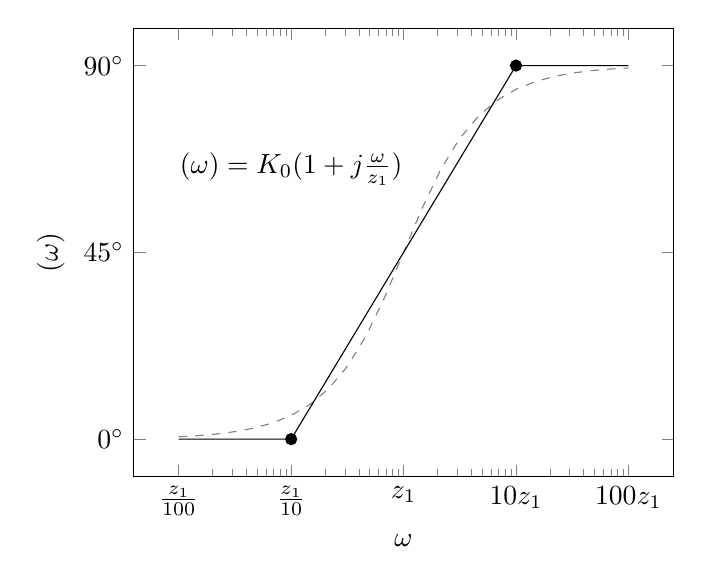
\begin{tikzpicture}
\begin{semilogxaxis}[ytick={0,45,90},yticklabels={$0^{\circ}$,$45^{\circ}$,$90^{\circ}$},xtick={1,10,100,1000,10000},xticklabels={$\frac{z_1}{100}$,$\frac{z_1}{10}$,$z_1$,$10z_1$,$100z_1$},xlabel={$\omega$},ylabel={$\phase{\bH(\omega)}$}]
\addplot[mark=none,color=gray,dashed,domain=1:10000]{atan(x/100)};
\addplot[mark=none,color=black] coordinates {(1,0) (10,0)  (1000,90) (10000,90)};
\addplot[mark=*,color=black] coordinates {(10,0) };
\addplot[mark=*,color=black] coordinates {(1000,90) };
\addplot[mark=none,color=black] coordinates {(10,65) }node[]{$\bH(\omega)=K_0(1+j\frac{\omega}{z_1})$};
\end{semilogxaxis}
\end{tikzpicture}
\caption{ایک صفر والے تفاعل کا بوڈا زاویائی خط۔}
\label{شکل_تعددی_زاویائی_بوڈا_ایک_صفر_الف}
\end{figure}
%================
\ابتدا{مثال}
تبادلی تفاعل \عددی{\bH(\omega)=\frac{50}{1+j\frac{\omega}{300}}} کا زاویائی بوڈا خط کھینچیں۔

حل:اس تفاعل کا زاویہ ذیل ہے جہاں کونا \عددی{\omega=\SI{300}{\radian\per\second}} پر پایا جاتا ہے۔
\begin{align}
\phase{\bH(\omega)}=\frac{1}{\phase{\tan^{-1} \frac{\omega}{300}}}=\phase{-\tan^{-1}\frac{\omega}{300}}
\end{align}
اس تفاعل کو شکل \حوالہ{شکل_تعددی_زاویائی_بوڈا_ایک_قطب_الف} میں ہلکی سیاہی میں نقطہ دار لکیر سے دکھایا گیا ہے۔

بوڈا خط میں کونے سے دس گنا کم تعدد پر زاویہ \عددی{0^{\circ}} اور کونے سے دس گنا زیادہ تعدد پر زاویہ \عددی{-90^{\circ}} چنتے ہوئے ان نقطوں کو سیدھے خط سے ملایا جاتا ہے۔یوں \عددی{\omega=\SI{30}{\radian\per\second}} پر \عددی{0^{\circ}} اور  \عددی{\omega=\SI{3000}{\radian\per\second}} پر \عددی{90^{\circ}} چنتے ہوئے انہیں سیدھے لکیر سے ملایا گیا ہے۔مزید  \عددی{\omega=\SI{30}{\radian\per\second}} سے کم تعدد پر زاویہ \عددی{0^{\circ}} ہی رکھا جاتا ہے جبکہ \عددی{\omega=\SI{3000}{\radian\per\second}} سے زیادہ تعدد پر زاویہ \عددی{-90^{\circ}} رکھا جاتا ہے۔بوڈا زاویائی خط کو شکل  \حوالہ{شکل_تعددی_زاویائی_بوڈا_ایک_قطب_الف} میں گہری سیاہی میں دکھایا گیا ہے۔
\begin{figure}
\centering
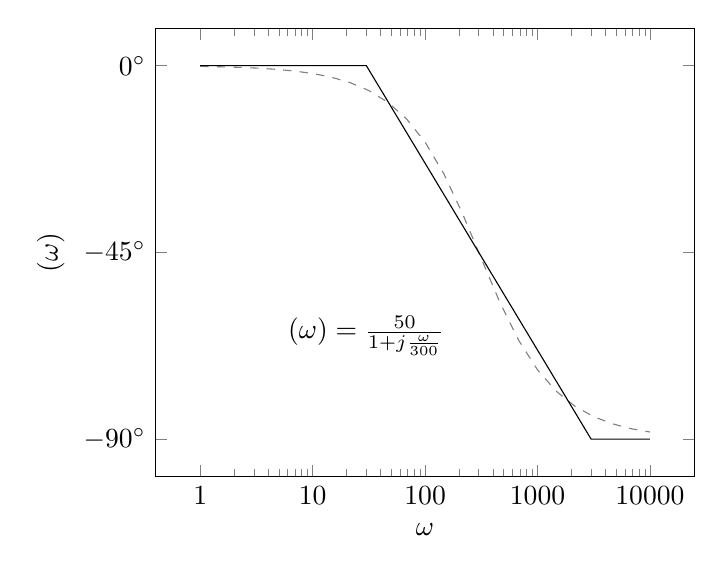
\begin{tikzpicture}
\begin{semilogxaxis}[ytick={0,-45,-90},yticklabels={$0^{\circ}$,$-45^{\circ}$,$-90^{\circ}$},xtick={1,10,100,1000,10000},xticklabels={$1$,$10$,$100$,$1000$,$10000$},xlabel={$\omega$},ylabel={$\phase{\bH(\omega)}$}]
\addplot[mark=none,color=gray,dashed,domain=1:10000]{-atan(x/300)};
\addplot[mark=none,color=black] coordinates {(1,0) (30,0)  (3000,-90) (10000,-90)};
\addplot[mark=none,color=black] coordinates {(30,-65) }node[]{$\bH(\omega)=\frac{50}{1+j\frac{\omega}{300}}$};
\end{semilogxaxis}
\end{tikzpicture}
\caption{ایک قطب والے تفاعل کا بوڈا زاویائی خط۔}
\label{شکل_تعددی_زاویائی_بوڈا_ایک_قطب_الف}
\end{figure}

یوں کونے \عددی{(\omega=\SI{300}{\radian\per\second})} پر، کونے سے دس گنا زیادہ تعدد \عددی{(\omega=\SI{3000}{\radian\per\second})} پر اور کونے سے دس گنا کم تعدد \عددی{(\omega=\SI{30}{\radian\per\second})} پر زاویے درج ذیل حاصل ہوتے ہیں۔
\begin{align*}
\phase{\bH(200)}&=\phase{-\tan^{-1} \frac{300}{300}}=\phase{-45^{\circ}}\\[0.5ex]
\phase{\bH(2000)}&=\phase{-\tan^{-1} \frac{3000}{300}}=\phase{-84.3^{\circ}}\\[0.5ex]
\phase{\bH(20)}&=\phase{-\tan^{-1} \frac{30}{300}}=\phase{-5.7^{\circ}}
\end{align*}

\انتہا{مثال}
%=========================
\ابتدا{مثال}
تبادلی تفاعل \عددی{\bH()=\frac{j10\omega}{(1+j\frac{\omega}{100})(1+j\frac{\omega}{10000})}} کا مقداری بوڈا خط کھینچیں۔

حل:اس تفاعل کی حتمی قیمت 
\begin{align*}
\abs{\bH(\omega)}=\frac{10\omega}{\sqrt{1+\frac{\omega^2}{100^2}}\sqrt{1+\frac{\omega^2}{10000^2}}}
\end{align*}
کو ڈیسی بیل میں لکھتے ہیں۔
\begin{align}\label{مساوات_تعددی_چار_رکنی_بوڈا}
20\log_{10} 10 +20\log_{10}\omega -20\log_{10}\sqrt{1+\frac{\omega^2}{100^2}} -20\log_{10}\sqrt{1+\frac{\omega^2}{10000^2}}
\end{align}
مساوات \حوالہ{مساوات_تعددی_چار_رکنی_بوڈا} کا پہلا رکن \عددی{\SI{20}{\deci\bel}} کا مستقل ہے۔اس کا دوسرا رکن \عددی{\omega=\SI{1}{\radian\per\second}} پر \عددی{\SI{0}{\deci\bel}} کے برابر ہے جبکہ اس تعدد سے زیادہ تعدد پر بتدریج بیس ڈیسی بیل فی دہائی بڑھتا ہے۔تیسرے اور چوتھے ارکان کے بوڈا خط بالترتیب \عددی{\SI{100}{\radian\per\second}}  اور \عددی{\SI{10}{\kilo\radian\per\second}} تعدد پر منفی بیس ڈیسی بیل فی دہائی گھٹنا شروع ہوتے ہیں۔ان تمام ارکان کو شکل \حوالہ{شکل_تعددی_زاویائی_بوڈا_ایک_صفر_دو_قطب_الف}-الف اور ان کا مجموعہ شکل-ب میں دکھایا گیا ہے۔
\begin{figure}
\centering
\begin{subfigure}{1\textwidth}
\centering
\begin{tikzpicture}
\begin{semilogxaxis}[ytick={-40,-20,0,20,40,60},yticklabels={$\SI{-40}{\deci\bel}$,$\SI{-20}{\deci\bel}$,$\SI{0}{\deci\bel}$,$\SI{20}{\deci\bel}$,$\SI{40}{\deci\bel}$,$\SI{60}{\deci\bel}$},xtick={0.1,1,10,100,1000,10000,100000},xticklabels={$10^{-1}$,$10^0$,$10^1$,$10^2$,$10^3$,$10^4$,$10^5$},xlabel={$\omega(\si{\radian\per\second})$},ylabel={$\abs{\bH(\omega)}$}]
%\addplot[mark=none,color=gray,dashed,domain=1:10000]{-atan(x/300)};
\addplot[mark=none,color=black] coordinates {(0.1,20) (100000,20)};
\addplot[mark=none,color=black]coordinates{(0.1,0) (1,0) (100,40)};
\addplot[mark=none,color=black]coordinates{(0.1,0) (100,0) (10000,-40)};
\addplot[mark=none,color=black]coordinates{(0.1,0) (10000,0) (100000,-20)};
\end{semilogxaxis}
\end{tikzpicture}
\caption*{(الف)}
\end{subfigure}
\begin{subfigure}{1\textwidth}
\centering
\begin{tikzpicture}
\begin{semilogxaxis}[ytick={-40,-20,0,20,40,60},yticklabels={$\SI{-40}{\deci\bel}$,$\SI{-20}{\deci\bel}$,$\SI{0}{\deci\bel}$,$+\SI{20}{\deci\bel}$,$+\SI{40}{\deci\bel}$,$+\SI{60}{\deci\bel}$},xtick={0.1,1,10,100,1000,10000,100000},xticklabels={$10^{-1}$,$10^0$,$10^1$,$10^2$,$10^3$,$10^4$,$10^5$},xlabel={$\omega(\si{\radian\per\second})$},ylabel={$\abs{\bH(\omega)}$}]
%\addplot[mark=none,color=gray,dashed,domain=1:10000]{-atan(x/300)};
\addplot[mark=none,color=black] coordinates {(0.1,20) (1,20) (100,60) (10000,60) (100000,40)};
\end{semilogxaxis}
\end{tikzpicture}
\caption*{(ب)}
\end{subfigure}
\caption{ایک صفر اور دو قطب والے تفاعل کا بوڈا مقداری خط۔}
\label{شکل_تعددی_زاویائی_بوڈا_ایک_صفر_دو_قطب_الف}
\end{figure}

ہمیں عموماً درمیانی تعدد پر بوڈا خط میں زیادہ دلچسپی ہوتی ہے۔ایسی صورت میں بوڈا مقداری خط درمیانی تعدد \عددی{(\SI{100}{\radian\per\second} <\omega<\SI{10}{\kilo\radian\per\second})} سے شروع کرنا بہتر ثابت ہوتا ہے۔دونوں کونوں سے دور یعنی \عددی{\omega\ll \SI{10}{\kilo\radian\per\second}} اور \عددی{\omega \gg \SI{100}{\radian\per\second}} پر  \عددی{1+\tfrac{\omega^2}{100^2}\approx \tfrac{\omega^2}{100^2}} اور \عددی{1+\tfrac{\omega^2}{10000^2}=1} لکھتے ہوئے درج ذیل لکھا جا سکتا ہے
\begin{align*}
\abs{\bH(\omega)}=\frac{10\omega}{\left(\sqrt{\frac{\omega^2}{100^2}}\right)\left(\sqrt{1}\right)}=1000 
\end{align*}
لہٰذا درمیانی تعددی پٹی پر ڈیسی بیل میں مقدار درج ذیل ہو گی
\begin{align*}
20\log_{10}\abs{\bH(\omega)}=20\log_{10} 1000=\SI{60}{\deci\bel} 
\end{align*}
 جسے شکل \حوالہ{شکل_تعددی_زاویائی_بوڈا_ایک_صفر_دو_قطب_الف}-ب میں \عددی{\omega=\SI{100}{\radian\per\second}} تا \عددی{\SI{10}{\kilo\radian\per\second}} دکھایا گیا ہے۔چونکہ حقیقت میں پست تعددی کونے  سے کم تعدد پر مقدار مسلسل بیس ڈیسی بیل فی دہائی بڑھتے ہوئے عین \عددی{\omega=\SI{100}{\radian\per\second}}  پر \عددی{\SI{60}{\deci\bel}} تک پہنچتی ہے لہٰذا پست تعددی کونے سے بیس ڈیسی بیل فی دہائی ڈھلوان کا خط کھینچیں۔اسی طرح بلند تعدد کونے پر بھی بیس ڈیسی بیل فی دہائی ڈھلوان کا خط کھینچیں۔یوں مکمل بوڈا خط حاصل ہو گا۔ 
\انتہا{مثال}
%=================
\ابتدا{مثال}\شناخت{مثال_تعددی_چالیس_ڈیسی_بیل_ڈھلوان}
تبادلی تفاعل \عددی{\bH(\omega)=\frac{10\left(1+j\frac{\omega}{10}\right)\left(1+j\frac{\omega}{1000}\right)}{\left(1+j\frac{\omega}{\num{100000}}\right)^2 \left(1+j\frac{\omega}{\num{1000000}}\right)^2}} کا مقداری بوڈا خط کھینچیں۔

حل:تفاول کی مقدار کو ڈیسی بیل میں لکھتے ہیں۔ان کا مجموعہ شکل \حوالہ{شکل_تعددی_چالیس_ڈیسی_بیل_ڈھلوان} میں دکھایا گیا ہے۔
\begin{multline*}
20\log_{10}\abs{\bH(\omega)}=20\log_{10} 10 +20\log_{10} \sqrt{1+\frac{\omega}{10^2}}+20\log_{10}\sqrt{1+\frac{\omega^2}{10^6}} \\
-40\log_{10}\sqrt{1+\frac{\omega^2}{10^10}}-40\log_{10}\sqrt{1+\frac{\omega^2}{10^{12}}}
\end{multline*}
یہاں \عددی{\SI{10}{\radian\per\second}} پر درج بالا مساوات کا دوسرا جزو بیس ڈیسی بیل فی دہائی بڑھنا شروع ہو جات ہے جبکہ تیسرا جزو اسی شرح سے \عددی{\SI{1000}{\radian\per\second}} پر بڑھنا شروع ہوتا ہے۔یوں ان کا مجموعہ لیتے ہوئے \عددی{\SI{1000}{\radian\per\second}} تعدد سے خط کی ڈھلوان \عددی{\SI{40}{\deci\bel}} فی دہائی ہو گی۔اسی طرح \عددی{\SI{100}{\kilo\radian\per\second}} پر چھوتا جزو \عددی{\SI{40}{\deci\bel}} فی دہائی سے گھٹنا شروع ہوتا ہے جو دوسرے اور تیسرے اجزاء کو ختم کرتا ہے لہٰذا بوڈا خط برقرار \عددی{\SI{140}{\deci\bel}} پر رہتا ہے۔آخر کار \عددی{\SI{1}{\mega\radian\per\second}} پر پانچواں جزو چالیس ڈیسی بیل فی دہائی سے گھٹنا شروع ہوتا ہے۔ 
\begin{figure}
\centering
\begin{tikzpicture}
\begin{semilogxaxis}[ytick={0,20,40,60,80,100,120,140,160},yticklabels={$\SI{0}{\deci\bel}$,$\SI{20}{\deci\bel}$,$\SI{40}{\deci\bel}$,$\SI{60}{\deci\bel}$,$\SI{80}{\deci\bel}$,$\SI{100}{\deci\bel}$,$\SI{120}{\deci\bel}$,$\SI{140}{\deci\bel}$,$\SI{160}{\deci\bel}$},xlabel={$\omega(\si{\radian\per\second})$},ylabel={$\abs{\bH(\omega)}$}]
\addplot[mark=none,color=black] coordinates {(1,20) (10,20) (1000,60) (100000,140) (1000000,140) (10000000,100)};
\addplot[mark=none,color=black] coordinates {(200,40)}node[right]{$\SI{20}{\deci\bel}/\text{دہائی}$};
\addplot[mark=none,color=black] coordinates {(3000,80)}node[left]{$\SI{40}{\deci\bel}/\text{دہائی}$};
\addplot[mark=none,color=black] coordinates {(10000000,100)}node[left]{$\SI{-40}{\deci\bel}/\text{دہائی}$};
\end{semilogxaxis}
\end{tikzpicture}
\caption{مثال \حوالہ{مثال_تعددی_چالیس_ڈیسی_بیل_ڈھلوان} کا مقداری بوڈا خط۔}
\label{شکل_تعددی_چالیس_ڈیسی_بیل_ڈھلوان}
\end{figure}

\انتہا{مثال}
%==================
